\documentclass[a4paper,11pt]{article}

% FILL OUT THE DETAILS BELOW:
\author{
\begin{tabular}{cc}
Ruben Dunnewolt (661890) & Joost Fitton (659382) \\
Luuk Jille (703714)     & Kevin Smit (707087)
\end{tabular}
}
\title{The Post-1994 Breakdown of Equity Premium Combination Forecasts:
A Variance Decomposition Approach}
% \date{An optional custom date, the default is today}
\newcommand{\program}{Econometrics \& Operations Research}
\newcommand{\supervisor}{Sam van Meer}

\usepackage[british]{babel} % Use British English
\usepackage[onehalfspacing]{setspace} % Increase line spacing
\usepackage[margin=2.5cm]{geometry} % Modify margins
\usepackage{graphicx,booktabs} % Packages for images and tables
\usepackage[authoryear]{natbib} % APA-style author-year citations

% ADD YOUR OWN PACKAGES HERE
\usepackage{array}
\usepackage{threeparttable}
\usepackage{siunitx}
\usepackage{amsmath,amssymb,amsfonts}
\usepackage[counterclockwise]{rotating}
\usepackage{hyperref}
\usepackage{float}
\usepackage[T1]{fontenc}
\usepackage{titlesec}
\usepackage{microtype}
\usepackage{enumitem}
\usepackage{subcaption}
\usepackage{appendix}

\begin{document}

\begin{titlepage}
\makeatletter
\begin{center}
	\textsc{Erasmus University Rotterdam}
	\par \textsc{Erasmus School of Economics}
	\par Seminar in Investing \program

	\vspace{0.5cm} \hrule height .08em \bigskip
	\par\huge\@title\bigskip
	\par\Large\@author\bigskip
	\hrule height .08em\normalsize
	
	\vspace{1cm} % small controlled space instead of stretch

\includegraphics[width=\textwidth,height=0.15\textheight,keepaspectratio]{eur}

\vspace{0.8cm}
\begin{tabular}{ll}
	
		\toprule
		Supervisor: & \supervisor\\
		Date final version: & \@date\\
		\bottomrule
	\end{tabular}
    \vspace{0.4cm}
\begin{abstract}
\end{abstract}
\end{center}
\makeatother

\end{titlepage}

\section{Introduction}

\newpage
\section{Forecast Error Decomposition and Diagnostic Evidence}
\label{sec:decomposition}

This section develops the algebraic framework we use to diagnose combination forecast performance. Section 3.1 fixes notation and states the combination forecast problem. Section 3.2 decomposes the forecast error covariance matrix via the law of total variance. Section 3.3 states the predictions each component delivers for combination performance. Section 3.4 defines the rolling diagnostic statistics that operationalize the decomposition. Section 3.5 states the structural break tests we apply to detect regime shifts.

\subsection{Setup}

Let $r_{t+1}$ denote the equity premium at time $t+1$ and $\mathcal{F}_t$ the information set available at time $t$. For each predictor $i = 1, \ldots, N$, a bivariate predictive regression estimated recursively on data through $t$ yields the forecast

\begin{equation*}
\hat{r}_{i,t+1} = \hat{\alpha}_{i,t} + \hat{\beta}_{i,t} x_{i,t},
\end{equation*}

\noindent which is $\mathcal{F}_t$-measurable by construction. Collect the $N$ forecasts in $\hat{\mathbf{r}}_{t+1} = (\hat{r}_{1,t+1}, \ldots, \hat{r}_{N,t+1})'$ and the forecast errors $e_{i,t+1} = r_{t+1} - \hat{r}_{i,t+1}$ in $\mathbf{e}_{t+1} = r_{t+1}\iota - \hat{\mathbf{r}}_{t+1}$, where $\iota$ is the $N \times 1$ vector of ones. The forecast error covariance matrix is $\Sigma_e = \mathrm{Var}(\mathbf{e}_{t+1})$.

The equal-weighted combination forecast of Rapach, Strauss, and Zhou (2010) is

\begin{equation*}
\bar{r}_{t+1} = \frac{1}{N} \iota' \hat{\mathbf{r}}_{t+1},
\end{equation*}

\noindent with combination error $\bar{e}_{t+1} = N^{-1} \iota' \mathbf{e}_{t+1}$ and combination MSFE

\begin{equation}
\mathrm{MSFE}(\bar{r}) = E[\bar{e}_{t+1}^2] = \frac{1}{N^2} \iota' \Sigma_e \iota. \label{eq:1}
\end{equation}

\noindent Equation \eqref{eq:1} shows that $1/N$ combination MSFE is fully determined by $\Sigma_e$. Understanding when $1/N$ performs well therefore reduces to understanding the structure of $\Sigma_e$.

\subsection{Decomposition of the Forecast Error Covariance Matrix}

Each individual forecast error can be written as the difference between the realised
return $r_{t+1}$ and the model-specific prediction $\hat{r}_{i,t+1}$:
\begin{equation}
    e_{i,t+1} = r_{t+1} - \hat{r}_{i,t+1}.
\end{equation}
Applying the law of total variance $\mathrm{Var}(r_{t+1}) =
\mathbb{E}[\mathrm{Var}(r_{t+1} \mid \mathcal{F}_t)] +
\mathrm{Var}(\mathbb{E}[r_{t+1} \mid \mathcal{F}_t])$ to the realised return,

\begin{equation*}
\mathrm{Var}(r_{t+1}) = E[\mathrm{Var}(r_{t+1} \mid \mathcal{F}_t)] + \mathrm{Var}(E[r_{t+1} \mid \mathcal{F}_t]),
\end{equation*}

\noindent the forecast error covariance matrix decomposes as

\begin{equation}
\Sigma_e = \underbrace{E[\mathrm{Var}(r_{t+1} \mid \mathcal{F}_t)] \, \iota\iota'}_{\text{common-return component}} + \underbrace{\mathrm{Var}\!\left(E[r_{t+1} \mid \mathcal{F}_t]\,\iota - \hat{\mathbf{r}}_{t+1}\right)}_{\text{cross-forecast component}}. \label{eq:2}
\end{equation}

The first term captures the part of return variation that is unpredictable given $\mathcal{F}_t$; because the forecasts $\hat{\mathbf{r}}_{t+1}$ are $\mathcal{F}_t$-measurable, they do not appear in it. Since every forecast error is subject to the same unpredictable return shock, this term enters every element of $\Sigma_e$ with coefficient one, reflected in the $\iota\iota'$ structure.

Expanding the cross-forecast component via the standard variance expansion yields five terms:

\begin{equation}\label{eq:cross-forecast-expand-resize}
\resizebox{\textwidth}{!}{$
    \Sigma_e =
    \underbrace{\mathbb{E}[\mathrm{Var}(r_{t+1} \mid \mathcal{F}_t)]\iota\iota'}_{\text{(i) common-return component}}
    + \underbrace{\mathrm{Var}(\mathbb{E}[r_{t+1} \mid \mathcal{F}_t])\iota\iota'}_{\text{(ii)}}
    - \underbrace{\iota\,\mathrm{Cov}(\mathbb{E}[r_{t+1} \mid \mathcal{F}_t], \hat{\mathbf{r}}_{t+1})'}_{\text{(iii)}}
    - \underbrace{\mathrm{Cov}(\mathbb{E}[r_{t+1} \mid \mathcal{F}_t], \hat{\mathbf{r}}_{t+1})\,\iota'}_{\text{(iv)}}
    + \underbrace{\mathrm{Var}(\hat{\mathbf{r}}_{t+1})}_{\text{(v)}}
$}
\end{equation}

To interpret these terms, write the realized return as $r_{t+1} = F(\mathcal{F}_t) + \varepsilon_{t+1}$, where $F(\mathcal{F}_t) = E[r_{t+1} \mid \mathcal{F}_t]$ is the true conditional expectation and $\varepsilon_{t+1}$ is the innovation satisfying $E[\varepsilon_{t+1} \mid \mathcal{F}_t] = 0$. The conditional expectation is the part of return variation that is predictable in principle; the innovation is the part no model can recover.

\textit{Term (i): Innovation variance.} The term $E[\mathrm{Var}(r_{t+1} \mid \mathcal{F}_t)] = \mathrm{Var}(\varepsilon_{t+1})$ is irreducible by construction. The innovation is orthogonal to every $\mathcal{F}_t$-measurable quantity, hits every forecast error with equal force, and cannot be diversified across forecasts.

It is important to clarify what we mean when we call a forecasting error ``irreducible.'' In pure statistical theory, term (i) is fixed: this random shock (the innovation, $\varepsilon_{t+1}$) is fundamentally impossible to predict using the information we currently have ($\mathcal{F}_t$). In reality, however, the boundary between what is reducible and irreducible depends entirely on the specific variables we use to approximate the true conditional expectation, $F(\mathcal{F}_t)$. 

If we had access to a better, richer dataset, some of the error we currently assign to term (i) might actually shift into term (ii) and turn out to be predictable. Therefore, our estimates of the innovation variance should really just be seen as the limits of our current data. It doesn't prove that the equity premium is fundamentally impossible to predict; it just provides an upper bound on the predictive power of the specific variables we chose to use.

\textit{Term (ii): Conditional mean variance}\textbf{.} The term $\mathrm{Var}(E[r_{t+1} \mid \mathcal{F}_t])$ represents the part of return variation that is predictable in principle. A forecaster who knew $F(\mathcal{F}_t)$ exactly could set $\hat{r}_{i,t+1} = F(\mathcal{F}_t)$ for every $i$, eliminating the contribution of this term to forecast errors entirely. In practice $F(\mathcal{F}_t)$ is unobserved and must be approximated. When predictors are genuinely informative this term contributes to reducing forecast errors; when predictors lose their connection to realized returns the approximation fails and this term behaves like term (i). It is reducible in principle, but we cannot actually exploit this predictability if the model we use to approximate the true relationship is poor.

\textit{Terms (iii) and (iv): Forecast-return cross-covariances.} These terms simply measure how closely each individual forecast moves together with the actual, realized return. If a predictor does a good job of tracking the true conditional expectation, $F(\mathcal{F}_t)$, its forecast will move in the same direction as the actual return, $r_{t+1}$. Because it successfully captures more of the predictable movement, it leaves behind less unexplained noise in its forecast error, $e_{i,t+1}$.

Since this improvement is unique to each specific predictor, it reduces the shared error across all forecasts. Furthermore, if different predictors capture different pieces of the true relationship, they will make different kinds of mistakes. This lowers the correlations between their errors, shrinking the off-diagonal elements of the forecast error covariance matrix, $\Sigma_e$. These terms are reducible in principle, and maximizing this co-movement is the main goal of standard forecasting methods that rely on individual predictive models.

\textit{Term (v): Forecast covariance.} The term $\mathrm{Var}(\hat{\mathbf{r}}_{t+1})$ measures how much the individual forecasts move together. If the forecasts are highly correlated, they tend to make the same mistakes at the same time, which inflates the total forecast error matrix, $\Sigma_e$. This is the component over which a combination method has the most direct control: diversifying across forecasts that are not perfectly correlated reduces its contribution to total forecast error variance.

It is useful to separate forecast covariance from predictor covariance. With bivariate forecasts $\hat{r}_{i,t+1} = \hat{\alpha}_{i,t} + \hat{\beta}_{i,t} x_{i,t}$,

\begin{equation*}
\mathrm{Cov}(\hat{r}_{i,t+1}, \hat{r}_{j,t+1}) = \hat{\beta}_{i,t}\hat{\beta}_{j,t} \mathrm{Cov}(x_{i,t}, x_{j,t}),
\end{equation*}

\noindent so forecast covariance inherits predictor covariance, multiplied by the slopes each predictor earns from its in-sample relation to returns. Two distinct forces can drive $\mathrm{Var}(\hat{\mathbf{r}}_{t+1})$ upward: predictors becoming more correlated, or bivariate slopes converging so that forecasts align even when the underlying predictors remain distinct. The diagnostics in Section 3.5 address both forces jointly at the forecast level, which is the level at which combination methods operate.

\textit{Collecting terms.} Because neither term (i) nor term (ii) can be acted upon directly in our forecasting framework, we combine them using $E[\mathrm{Var}(r_{t+1} \mid \mathcal{F}_t)] + \mathrm{Var}(E[r_{t+1} \mid \mathcal{F}_t]) = \mathrm{Var}(r_{t+1})$, yielding the three-component decomposition that forms the basis of our empirical analysis:

\begin{equation}
\Sigma_e = \underbrace{\sigma_{r_{t+1}}^2 \, \iota\iota'}_{\text{return variance}} - \underbrace{\iota\boldsymbol{\sigma}_{r,\hat{r}}' + \boldsymbol{\sigma}_{r,\hat{r}}\iota'}_{\text{forecast-return cross-covariance}} + \underbrace{\mathrm{Var}(\hat{\mathbf{r}}_{t+1})}_{\text{forecast covariance}}, \label{eq:3-part-decomp}
\end{equation}

where $\sigma_{r_{t+1}}^2 = \mathrm{Var}(r_{t+1})$ and $\boldsymbol{\sigma}_{r, \hat{r}} = \mathrm{Cov}(E[r_{t+1} \mid \mathcal{F}_t], \hat{\mathbf{r}}_{t+1})$ is the $N \times 1$ vector of forecast-return cross-covariances.

The decomposition \eqref{eq:3-part-decomp} looks like error accounting, but it it directly reflects standard ways to measure forecasting success.Specifically, the cross-covariance vector $\boldsymbol{\sigma}_{r,\hat{r}}$ acts like a theoretical version of the out-of-sample $R^2$: When $\sigma_{r,\hat{r}_i} > 0$, the forecast $\hat{r}_{i,t+1}$ moves with $r_{t+1}$ and contains directly exploitable signal; when $\sigma_{r,\hat{r}_i} = 0$, the forecast is uninformative and the optimal choice collapses to the historical mean; when $\sigma_{r,\hat{r}_i} < 0$, the forecast points the wrong way, meaning information is present but inverted and a sign-flipped version $-\hat{r}_{i,t+1}$ would be informative.
This distinction is crucial because none of the combination methods we evaluate in Section 4 flip signs based on recent performance: 1/N, DMSFE, and sPCA all take forecasts at face value, and while rolling OLS and D-OLS re-estimate slopes in each window, they can only track sign changes if the new sign is stable within the estimation window. A predictor whose forecast has $\sigma_{r,\hat{r}_i} < 0$ in a given sample therefore contributes noise, not signal, to every combination scheme we consider. Failure of a combination forecast under this class of methods reflects either a collapse in $|\boldsymbol{\sigma}_{r,\hat{r}}|$ (genuine loss of information content) or a sign reversal that the methods cannot recover (information is present but unrecoverable by sign-preserving combinations). Both are empirically distinguishablethe, the first shows up as cross-covariances shrinking toward zero, the second as sign flips with preserved magnitude.

\subsection{Decomposition of Combination MSFE}

\noindent Substituting Equation \ref{eq:3-part-decomp} into Equation \ref{eq:1} and using $\iota'\iota = N$, 

\begin{equation}
    \mathrm{MSFE}(\bar{r}) = \sigma_{r_{t+1}}^2 - 2\bar{\sigma}_{r,\hat{r}} + \bar{v},
\end{equation}
\noindent where

$$ \bar{\sigma}_{r,\hat{r}} \equiv \frac{1}{N} \iota' \boldsymbol{\sigma}_{r,\hat{r}}, \qquad \bar{v} \equiv \frac{1}{N^2} \iota' \mathrm{Var}(\hat{\mathbf{r}}_{t+1}) \iota, $$

\noindent are the averages across forecasts of the forecast-return cross-covariance and of the pairwise forecast covariance matrix (inclusive of the diagonal).

The prevailing-mean benchmark, which sets $\hat{r}_{t+1} = E[r_{t+1}]$,  has MSFE equal to $\sigma_{r_{t+1}}^2$. The combination forecast beats the benchmark if and only if
\begin{equation}
2\bar{\sigma}_{r,\hat{r}} > \bar{v}. \qquad     
\label{eq:decomp_ineq}
\end{equation}


Condition \eqref{eq:decomp_ineq} gives us a clear, intuitive rule: twice the average forecast-return covariance must be strictly greater than thethe average pairwise forecast covariance. Each side of the inequality corresponds to one channel through which $1/N$ can fail, and each channel suggests different corrective methods. Diagnosing which channel drives combination forecast failure is therefore the natural first step in any attempt to repair it.

\subsection{What Does Each Component Predict for Combination Performance?}
\label{subsec:component_meaning}
\noindent The decomposition generates testable hypotheses about what must be changing in the data if combination forecast performance is deteriorating. We state them in terms of the underlying components (i)--(v) from \ref{eq:cross-forecast-expand-resize}, because these are mutually orthogonal. The collected components in \ref{eq:3-part-decomp} are more convenient empirically but bundle terms that carry opposite implications for combination forecasts.

\textit{Innovation-variance hypothesis.} If the genuinely unpredictable component of return variation, $E[\mathrm{Var}(r_{t+1} \mid \mathcal{F}_t)]$ , rises, then term (i) in \ref{eq:cross-forecast-expand-resize} rises uniformly. All forecasts are equally affected and no combination scheme can help, because the innovation is orthogonal to every $\mathcal{F}_t$-measurable forecast. Empirically, this shows as a proportional rise in realized squared forecast errors across all predictors, driven by unabsorbable market volatility.

\textit{Information-loss hypothesis.} If the absolute magnitudes, $|\sigma_{r,\hat{r}_i}|$, of the forecast-return cross-covariances (terms iii and iv) collapse toward zero, individual forecasts are genuinely losing their informational content regarding the realized return. As these negative terms in equation (4) shrink in absolute value, the total error covariance $\Sigma_e$ expands. Consequently, all combination methods deteriorate, as no reweighting scheme can extract a signal that no longer exists. 

Crucially, this information loss can occur even if the unconditional return variance, $\sigma_{r_{t+1}}^2$, is stable or falling. This happens if the predictable variation, $\mathrm{Var}(E[r_{t+1} \mid \mathcal{F}_t])$, is shrinking alongside an offsetting rise in the unpredictable innovation variance. Without an external reference measure of true predictability, our decomposition cannot empirically distinguish between two distinct causes for this shrinkage:
\begin{itemize}
    \item \textit{Predictor-specific failure:} The true predictable component of the market remains stable, but our specific set of variables has lost its grip on it.
    \item \textit{Structural failure:} The underlying predictable component of the equity premium has itself fundamentally contracted.
\end{itemize}

Both scenarios are consistent with our empirical evidence, but they carry different implications for the scope of the failure. Regardless of the underlying cause, the cross-sectional nature of the decline dictates how we might fix it: a \textit{homogeneous} decline across all predictors leaves no room for adaptive weighting, whereas a \textit{heterogeneous} decline creates an opportunity to concentrate weight on surviving signals.

\textit{Sign-reversal hypothesis.} If the cross-covariances $\sigma_{r,\hat{r}_i}$ flip signs but preserve their magnitude, the forecasts still contain valid information, but they point in the wrong direction. Mathematically, the previously negative terms in equation (4) turn positive, actively amplifying rather than reducing $\Sigma_e$. This failure mode is conceptually distinct from true information loss: the signal is perfectly recoverable if a method explicitly flips the sign (e.g., using $-\hat{r}_{i,t+1}$). However, standard methods like $1/N$, DMSFE, and sPCA take forecasts at face value. (While rolling OLS and D-OLS can track stable sign changes via slope re-estimation, they lag immediate flips). Therefore, within the class of combination methods we consider, sign reversal acts empirically like a loss of usable signal, despite requiring an entirely different theoretical remedy.

\textit{Redundancy hypothesis.} If the forecast covariance, $\mathrm{Var}(\hat{\mathbf{r}}_{t+1})$ (term v), increases, individual forecasts are converging. Equal-weighted schemes then spread mass across highly redundant signals, eroding the cross-sectional diversification benefit. This covariance inflation is the mechanism most commonly cited in the existing literature for the post-1994 deterioration in predictability.

Because these four hypotheses map to distinct mathematical components of equation (3), their empirical signatures are separable, even if multiple forces act simultaneously. The rolling diagnostics developed in the next subsection, combined with the individual $\rho_{i,t}^{(W)}$ series, are specifically designed to distinguish true information loss (shrinking magnitudes) from sign reversal (preserved magnitudes, flipped signs), and both from redundancy shifts.

\subsection{Diagnostic Statistics}

To track the three components over time, we construct two rolling correlation measures. Rolling windows allow detection of structural changes in the forecast error covariance structure without imposing a single breakpoint. Correlations rather than covariances normalise away scale effects and permit comparison across frequencies and subperiods. Over a window of $W$ observations ending at $t$, define

\begin{equation}
S^{fr}_t = \frac{1}{N} \sum_{i=1}^{N} \mathrm{corr}_{{t-W+1}:t}(r_{s+1}, \hat{r}_{i,s+1}), \label{eq:7}
\end{equation}

\begin{equation}
S^{p}_t = \frac{2}{N(N-1)} \sum_{i < j} \mathrm{corr}_{t-W+1:t}(\hat{r}_{i,s+1}, \hat{r}_{j,s+1}). \label{eq:8}
\end{equation}

The statistic $S^{fr}_t$ measures how well individual forecasts track the realized return on average. A persistent decline signals erosion of the information channel; a negative value means forecasts on average point in the wrong direction. The statistic $S^{p}_t$ measures average redundancy among forecasts. We compute each statistic using both Pearson and Spearman correlation. A high value means predictors are producing very similar forecasts, so equal weights offer little diversification benefit. The contrast between $S^{fr}_t$ and $S^{p}_t$ isolates which component of \eqref{eq:3-part-decomp} is moving.

To test whether changes in $S^{fr}_t$ are homogeneous or heterogeneous across predictors, we also compute the individual forecast-return correlation

\begin{equation}
\rho_{i,t}^{(W)} = \mathrm{corr}_{t-W+1:t}(r_{s+1}, \hat{r}_{i,s+1}) \label{eq:9}
\end{equation}

for each predictor separately. Homogeneous decline implies individual correlations move together; heterogeneous decline implies some predictors retain positive correlation while others deteriorate, creating scope for predictor-selection or predictor-weighting schemes to exploit the surviving signal.

\subsection{Structural Break Framework}

The decomposition in equation \eqref{eq:3-part-decomp} describes the underlying population moments.. If these moments shift at some point in the sample, combination forecast performance shifts with them, and rolling diagnostics pick up the change gradually as the window moves through the break. To test formally for regime change in the quantities that drive \ref{eq:3-part-decomp}, we apply two complementary procedures.

\textbf{Single-break test.} The Andrews (1993) sup-$F$ test checks for a single structural break at an unknown date. It uses a trimming parameter $\varepsilon$ to exclude the extreme ends of the sample (the outer $100\varepsilon\%$ of candidate break dates). We apply this test to three sets of regressions:
\begin{itemize}
    \item The equity premium (regressing $r_{t+1}$ on a constant).
    \item The $1/N$ combination forecast error, $\bar{e}_{t+1}$, which directly tests whether the combination's relative performance has shifted.
    \item The individual predictive regressions, $r_{t+1} = \alpha_i + \beta_i x_{i,t} + \varepsilon_{i,t+1}$, testing if the coefficients $(\alpha_i, \beta_i)$ break together for each of the $N$ predictors.
\end{itemize}

\textbf{Multiple-break test.} The sup-$F$ test struggles if there are multiple breaks, especially if they cancel each other out, and it can only identify a single break date. To address this, we supplement it with the Bai and Perron (2003) sequential procedure. This method sequentially tests whether $k$ breaks or $k+1$ breaks better describe the data (for $k = 0, 1, 2, \ldots$) and provides estimated break dates alongside their confidence intervals. We apply this procedure to the mean of the equity premium and the mean of the $1/N$ forecast error.

These two tests answer related but distinct questions. The sup-$F$ test asks if \textit{any} single break significantly improves the model. The Bai-Perron procedure asks \textit{how many} breaks the data actually support and exactly \textit{where} they are located. Used together, they allow us to cleanly classify the data into one of three structural environments: persistent stability, a single regime shift, or gradual and repeated regime change.

\section{Adaptive Forecasting Methods}

Section \ref{sec:decomposition} identified four hypotheses about why 1/N combination forecasts may deteriorate: rising innovation variance, loss of information magnitude, sign reversal, and rising forecast redundancy. No single adaptive method addresses all four, and the first, innovation variance, is irreducible by any forecasting procedure. This section introduces four methods that target the remaining three channels.

\subsection{Reweighting Methods}
These methods share the full-sample bivariate regressions used by $1/N$; they differ only in how the resulting $N$ forecasts are combined

\subsubsection{Scaled Principal Component Analysis (sPCA)}

Standard principal component analysis (PCA) extracts factors that explain predictor variance without regard to the forecasting target. \citet{huang2022scale} propose Scaled PCA (sPCA), which pre-weights each predictor by its in-sample slope coefficient on the target before extracting factors. This adjustment ensures that the resulting principal components prioritise the predictors' actual forecasting signal rather than their variance.

 First, we compute scaling weights. For each predictor $i = 1, \ldots, N$, estimate the bivariate predictive regression

$$r_{s+1} = \alpha_i + \beta_i x_{i,s} + \varepsilon_{i,s+1}, \qquad s = 1, \ldots, t-1, \qquad (1)$$

\noindent and collect the slope estimates in the diagonal matrix $\hat{\mathbf{B}}_t = \mathrm{diag}(\hat{\beta}_{1,t}, \ldots, \hat{\beta}_{N,t})$. Predictors with large in-sample slopes, i.e., large contributions to the forecast-return cross-covariance vector $\boldsymbol{\sigma}_{r,\hat{r}}$, receive large weights; predictors with near-zero slopes are shrunk toward zero.

Next, we scale the predictor matrix prior to extracting the principal components. Let $\mathbf{X}_t \in \mathbb{R}^{t \times N}$ denote the matrix of predictors over the expanding in-sample window. We form the scaled predictor matrix as:

\begin{equation}
\tilde{\mathbf{X}}_t = \mathbf{X}_t \hat{\mathbf{B}}_t, \label{eq:2}
\end{equation}

and extract the top $K$ principal components from the sample covariance of this scaled matrix. By defining the scaled covariance matrix as $\tilde{\mathbf{\Sigma}}_t = t^{-1} \tilde{\mathbf{X}}_t' \tilde{\mathbf{X}}_t$, we can rewrite the scaling operation to explicitly expose the two distinct mechanisms through which sPCA operates:

\begin{equation}
\tilde{\mathbf{\Sigma}}_t = \hat{\mathbf{B}}_t \left( t^{-1} \mathbf{X}_t' \mathbf{X}_t \right) \hat{\mathbf{B}}_t. \label{eq:3}
\end{equation}

Equation \eqref{eq:3} demonstrates that sPCA addresses both the cross-covariance and forecast-covariance channels simultaneously. These two effects enter the eigenvalue problem multiplicatively:
\begin{itemize}
    \item The inner matrix, $t^{-1} \mathbf{X}_t' \mathbf{X}_t$, represents the standard, unscaled predictor covariance. Taking its eigendecomposition naturally attenuates predictor redundancy (corresponding to term v of our decomposition).
    \item The outer matrices, $\hat{\mathbf{B}}_t$, re-weight this standard decomposition by the in-sample predictive slopes. This forces the retained factors to concentrate specifically on directions that are correlated with the realized returns (corresponding to terms iii and iv).
\end{itemize}

In short, sPCA structurally links the two remedies together: the scaling adjustment targets the predictive signal, the dimensionality reduction targets the redundancy, and both operate jointly within a single eigenvalue problem.

Let $\mathbf{V}_t \in \mathbb{R}^{N \times K}$ denote the matrix of top-$K$ eigenvectors of $\tilde{\mathbf{\Sigma}}_t$. The factor realizations are $\hat{\mathbf{F}}_t = \tilde{\mathbf{X}}_t \mathbf{V}_t$, and the forecast is

$$\hat{r}^{sPCA}_{t+1} = \hat{\theta}_{0,t} + \hat{\boldsymbol{\theta}}_t' \hat{\mathbf{f}}_t, \qquad (4)$$

where $\hat{\mathbf{f}}_t$ is the $K$-vector of factor realizations at time $t$ and $(\hat{\theta}_{0,t}, \hat{\boldsymbol{\theta}}_t)$ are OLS coefficients from regressing $r_{s+1}$ on $\hat{\mathbf{f}}_s$ over $s = 1, \ldots, t-1$.

We implement this procedure using an expanding window. To forecast the equity premium at each out-of-sample date $t$, the algorithm proceeds as follows:

\begin{enumerate}
    \item \textit{Compute scaling weights.} Using all data strictly before $t$, estimate $N$ bivariate predictive regressions of $r_{s+1}$ on a constant and the lagged predictor $x_{i,s}$, for $i = 1,\ldots,N$. Collect the OLS slope estimates $\hat{\beta}_{1,t},\ldots,\hat{\beta}_{N,t}$ in the diagonal matrix $\hat{\mathbf{B}}_t$. In the restricted specification, any slope whose sign conflicts with its theoretical prior is set to zero.

    \item \textit{Scale the predictor matrix.} Form $\tilde{\mathbf{X}}_t = \mathbf{X}_t \hat{\mathbf{B}}_t$, where $\mathbf{X}_t \in \mathbb{R}^{(t-1) \times N}$ contains the lagged predictor values over the expanding in-sample window.

    \item \textit{Standardise and extract factors.} Standardise each column of $\tilde{\mathbf{X}}_t$ to zero mean and unit variance. Apply PCA to the standardised matrix and retain the first $K_{\max} = 4$ principal components. Denote the in-sample factor matrix $\hat{\mathbf{F}}_t \in \mathbb{R}^{(t-1) \times K_{\max}}$.

    \item \textit{Forecast regression.} For each $K \in \{1,2,3,4\}$, regress $r_{s+1}$ on a constant and the first $K$ factors $\hat{\mathbf{F}}_t^{(K)} = [\hat{f}_{s,1},\ldots,\hat{f}_{s,K}]$ by OLS, yielding $(\hat{\theta}_{0,t}^{(K)}, \hat{\boldsymbol{\theta}}_t^{(K)})$.

    \item \textit{Out-of-sample projection.} Apply the same scaling weights $\hat{\mathbf{B}}_t$ and standardisation parameters to the time-$t$ predictor vector $\mathbf{x}_t$, then project onto the PCA loadings to obtain the out-of-sample factor vector $\hat{\mathbf{f}}_t^{(K)}$. The forecast for each $K$ is
    $$\hat{r}_{t+1}^{(K)} = \hat{\theta}_{0,t}^{(K)} + \hat{\boldsymbol{\theta}}_t^{(K)\prime} \hat{\mathbf{f}}_t^{(K)}.$$

    \item \textit{Model selection via accumulated out-of-sample AIC.} After each forecast date $t$, update the accumulated out-of-sample sum of squared errors for each $K$: $\mathrm{RSS}_K = \sum_{s} (r_{s+1} - \hat{r}_{s+1}^{(K)})^2$, where the sum runs over all prior out-of-sample observations. The accumulated out-of-sample AIC is
    $$\mathrm{AIC}_K = n_{\mathrm{oos}} \ln\!\left(\frac{\mathrm{RSS}_K}{n_{\mathrm{oos}}}\right) + 2(K+1),$$
    where $n_{\mathrm{oos}}$ is the number of out-of-sample observations accumulated so far. The best-AIC forecast at time $t$ selects the $K$ with the lowest accumulated $\mathrm{AIC}_K$ and uses the corresponding forecast $\hat{r}_{t+1}^{(K^*)}$. This adaptive selection allows the number of retained factors to vary over the evaluation period.
\end{enumerate}

\noindent We report results for fixed $K = 1,2,3,4$ as well as the best-AIC specification. The procedure is re-estimated at every out-of-sample date, so that scaling weights, standardisation parameters, PCA loadings, and forecast regression coefficients are all updated as new data arrive. By nesting all four factor sets within a single PCA fit per period, computational cost is kept proportional to the number of out-of-sample observations rather than the number of factor specifications.

\newpage
\begin{figure}[H]
    \centering
    
\includegraphics[width=1\linewidth]{Paper final Joost Copy/plot_S_fr_combined_monthly_unrestricted.png}
    \caption{monthly Sfr}
    \label{fig:placeholder}
\end{figure}
\begin{figure}[H]
    \centering
    
\includegraphics[width=1\linewidth]{Paper final Joost Copy/plot_S_fr_combined_quarterly_unrestricted.png}
    \caption{Quarterly Sfr}
    \label{fig:placeholder}
\end{figure}

\begin{figure}[H]
    \centering
    
\includegraphics[width=1\linewidth]{Paper final Joost Copy/plot_S_p_combined_monthly_unrestricted.png}
    \caption{monthly Sp}
    \label{fig:placeholder}
\end{figure}

\begin{figure}[H]
    \centering
    
\includegraphics[width=1\linewidth]{Paper final Joost Copy/plot_S_p_combined_quarterly_unrestricted.png}
    \caption{Quarterly Sp}
    \label{fig:placeholder}
\end{figure}


\begin{spacing}{1.0}
\begin{table}[H]
\centering
\caption{Variance Decomposition of the $1/N$ Forecast Error: Sub-Period Averages}
\label{tab:variance_decomposition}
\small
\renewcommand{\arraystretch}{1}
\begin{tabular}{@{}ll
                *{6}{S[table-format=-1.4]}@{}}
\toprule
& & \multicolumn{3}{c}{Quarterly} & \multicolumn{3}{c}{Monthly} \\
\cmidrule(r){3-5} \cmidrule(l){6-8}
{Component} & {Window}
& {1979--1993} & {1994--2022} & {$\Delta$}
& {1979--1993} & {1994--2022} & {$\Delta$} \\
\midrule
\multicolumn{8}{@{}l}{\textit{Panel A: Annualised variance of the equity premium}} \\
& {5-year}  & 0.0287 & 0.0248 & -0.0039 & 0.0276 & 0.0209 & -0.0067 \\
& {10-year} & 0.0284 & 0.0255 & -0.0029 & 0.0275 & 0.0220 & -0.0056 \\
& {15-year} & 0.0236 & 0.0261 &  0.0025 & 0.0242 & 0.0227 & -0.0015 \\[0.6ex]
\multicolumn{8}{@{}l}{\textit{Panel B: Forecast--return correlation ($S^{fr}_t$)}} \\
& {5-year}  &  0.0876 & -0.0475 & -0.1350 &  0.0296 & -0.0356 & -0.0652 \\
& {10-year} &  0.0571 & -0.0363 & -0.0934 &  0.0137 & -0.0289 & -0.0426 \\
& {15-year} &  0.0503 & -0.0273 & -0.0776 &  0.0052 & -0.0210 & -0.0263 \\[0.6ex]
\multicolumn{8}{@{}l}{\textit{Panel C: Forecast correlation ($S^{p}_t$)}} \\
& {5-year}  &  0.0104 &  0.0172 &  0.0068 &  0.0015 &  0.0150 &  0.0135 \\
& {10-year} & -0.0045 &  0.0153 &  0.0199 &  0.0043 &  0.0081 &  0.0038 \\
& {15-year} & -0.0281 &  0.0087 &  0.0369 & -0.0245 &  0.0018 &  0.0263 \\
\bottomrule
\end{tabular}
\vspace{0.4em}
\begin{minipage}{0.85\textwidth}
\footnotesize
\textit{Notes:} Sub-period averages of the rolling-window variance
decomposition components. Panel~A reports the annualised variance of the
equity premium. Panels~B and~C report the average forecast--return
correlation and forecast correlation, respectively. Window lengths are 5,
10, and 15~years. $\Delta$ denotes the difference between the post-1994
and pre-1994 averages.
\end{minipage}
\end{table}
\end{spacing}


\begin{spacing}{1.0}
\begin{table}[H]
\centering
\caption{Structural Break Tests}
\label{tab:break_tests}
\small
\renewcommand{\arraystretch}{1.05}
\begin{tabular}{@{}lcccl@{}}
\toprule
Test \& series & $k$ & $F(k)$ & 5\% c.v. & Estimated break(s) \\
\midrule
\multicolumn{5}{@{}l}{\textit{Panel A: sup-F (QLR), $\varepsilon = 0.15$, $q=1$}} \\
Equity premium (mean) & {--} & 4.24 & 5.86 & 1959-08 (n.s.) \\
$1/N$ forecast errors  & {--} & 5.85 & 5.86 & 1974-10 (n.s.) \\[0.3ex]
\midrule
\multicolumn{5}{@{}l}{\textit{Panel B: Bai--Perron, equity premium}} \\
& $k=1$ & 4.24 & 8.58 & 1959-08 \\
& $k=2$ & 4.85 & 7.22 & 1959-08, 2009-03 \\
& $k=3$ & 4.28 & 5.96 & 1959-08, 1997-08, 2009-03 \\
& $k=4$ & 4.77 & 4.99 & 1965-11, 1982-08, 1997-08, 2009-03 \\
& $k=5$ & 3.86 & 3.91 & 1959-08, 1971-03, 1982-08, 1997-08, 2009-03 \\[0.3ex]
\midrule
\multicolumn{5}{@{}l}{\textit{Panel C: Bai--Perron, $1/N$ forecast errors}} \\
& $k=1$ & 5.85 & 8.58 & 1974-10 \\
& $k=2$ & 5.69 & 7.22 & 2000-04, 2009-03 \\
& $k=3$ & 6.58{$^{**}$} & 5.96 & 1982-08, 2000-04, 2009-03 \\
& $k=4$ & 5.25{$^{**}$} & 4.99 & 1974-10, 1990-11, 2000-04, 2009-03 \\
& $k=5$ & 4.09{$^{**}$} & 3.91 & 1973-10, 1982-08, 1991-07, 2000-04, 2009-03 \\[0.3ex]
\midrule
\multicolumn{5}{@{}l}{\textit{Panel D: sup-F (QLR) on individual predictive regressions, $q=2$}} \\
D/P   & {--} & 11.72{$^{***}$} & 4.55 & 2009-03 \\
D/Y   & {--} &  9.89{$^{***}$} & 4.55 & 2009-03 \\
E/P   & {--} &  4.53{$^{*}$}   & 4.55 & 2009-03 \\
D/E   & {--} &  6.37{$^{***}$} & 4.55 & 2009-03 \\
SVAR  & {--} & 11.42{$^{***}$} & 4.55 & 2009-03 \\
B/M   & {--} &  5.63{$^{**}$}  & 4.55 & 2009-03 \\
NTIS  & {--} &  3.61            & 4.55 & 2003-04 \\
TBL   & {--} &  8.05{$^{***}$} & 4.55 & 1974-10 \\
LTY   & {--} &  7.22{$^{***}$} & 4.55 & 1974-10 \\
LTR   & {--} &  2.93            & 4.55 & 1959-08 \\
TMS   & {--} &  5.80{$^{**}$}  & 4.55 & 1975-07 \\
DFY   & {--} &  6.15{$^{**}$}  & 4.55 & 2009-03 \\
DFR   & {--} &  3.78{$^{*}$}   & 4.55 & 1969-07 \\
INFL  & {--} &  2.94            & 4.55 & 2008-08 \\
\bottomrule
\end{tabular}
\vspace{0.4em}
\begin{minipage}{0.95\textwidth}
\footnotesize
\textit{Notes:} Panel~A reports the \citet{Andrews1993} sup-F (QLR) test for
a single unknown break with trimming parameter $\varepsilon = 0.15$.
Critical values are for the sup-F statistic with $q=1$ (mean model):
10\%~=~5.86, 5\%~=~7.35. Panels~B and~C report the \citet{BaiPerron2003}
multiple-break procedure with $F(k)$ statistics and associated 5\%
critical values. $^{**}$ indicates significance at 5\%.
Panel~D reports sup-F tests on individual bivariate predictive regressions
($q = 2$). sup-F critical values for $q = 2$: 10\%~=~3.76,
5\%~=~4.55, 1\%~=~6.19.
$^{*}\!p < 0.10$, $^{**}\!p < 0.05$, $^{***}\!p < 0.01$.
\end{minipage}
\end{table}
\end{spacing}




\newpage
\section{Methods}
\newpage
\section{Data}
\newpage
\section{Results}


\begin{table}[H]
\centering
\caption{Out-of-Sample Performance of $1/N$ Combination Forecast for sPCA and DMFSE Weighting Scheme}
\label{tab:spca_results}
\small
\renewcommand{\arraystretch}{1}
\begin{tabular}{@{}l*{6}{S[table-format=-1.2,table-space-text-post={$^{***}$}]}@{}}
\toprule
 & \multicolumn{3}{c}{Quarterly} & \multicolumn{3}{c}{Monthly} \\
\cmidrule(lr){2-4} \cmidrule(lr){5-7}
{Method}
& {1979--2022} & {1979--1993} & {1994--2022} 
& {1979--2022} & {1979--1993} & {1994--2022} \\
\midrule
\multicolumn{7}{@{}l}{\textit{Panel A: Without \citet{campbellthompson2008} restrictions}} \\[0.3ex]
{1/N (RSZ)} 
& \bfseries \textbf{0.76{$^{*}$}} & \bfseries 2.62{$^{***}$} & -0.05 
& 0.16 & \bfseries 0.72{$^{**}$} & -0.14 \\[0.6ex]
{sPCA direct ($K=1$)} 
& -0.70 & -1.53 & -0.35 
& -0.36 & -0.58 & -0.25 \\
{sPCA direct ($K=3$)} 
& \bfseries -2.83{$^{*}$} & \bfseries \textbf{3.88{$^{**}$}} & -5.75 
& \bfseries \textbf{0.50{$^{**}$}} & \bfseries 1.95{$^{**}$} & -0.27 \\
{sPCA direct (K$_t$)} 
& -0.70 & -1.53 & -0.35 
& \bfseries 0.35{$^{**}$} & \bfseries \textbf{3.83{$^{***}$}} & -1.51 \\[0.6ex]
{DMFSE ($\delta = 1$)} 
& 0.58{$^{*}$} & 2.02{$^{**}$} & -0.04 
& 0.13 & 0.65{$^{**}$} & -0.14 \\
{DMFSE ($\delta = 0.99$)} 
& 0.57{$^{*}$} & 2.01{$^{**}$} & -0.05 
& 0.13 & 0.64{$^{**}$} & -0.14 \\
{DMFSE ($\delta = 0.95$)} 
& 0.57{$^{*}$} & 1.96{$^{**}$} & \textbf{-0.03} 
& 0.13 & 0.61{$^{**}$} & \textbf{-0.13} \\
\midrule
\multicolumn{7}{@{}l}{\textit{Panel B: With \citet{campbellthompson2008} restrictions}} \\[0.3ex]
{1/N (RSZ)} 
& \bfseries \textbf{0.90{$^{**}$}} & \bfseries 2.66{$^{***}$} & 0.13 
& \bfseries 0.23{$^{*}$} & \bfseries 0.81{$^{**}$} & -0.08 \\[0.6ex]
{sPCA direct ($K=1$)} 
& -0.35 & -1.22 & 0.02 
& -0.33 & -0.55 & -0.22 \\
{sPCA direct ($K=3$)} 
& -0.10 & \bfseries \textbf{7.48{$^{***}$}} & -3.40 
& \bfseries 0.79{$^{**}$} & \bfseries \textbf{2.99{$^{***}$}} & -0.39 \\
{sPCA direct (K$_t$)} 
& -0.35 & -1.22 & 0.02 
& \bfseries \textbf{1.03{$^{***}$}} & \bfseries 2.86{$^{***}$} & \textbf{0.04} \\[0.6ex]
{DMFSE ($\delta = 1$)} 
& 0.72{$^{*}$} & 2.05{$^{**}$} & 0.14 
& 0.20{$^{*}$} & 0.73{$^{**}$} & -0.08 \\
{DMFSE ($\delta = 0.99$)} 
& 0.71{$^{*}$} & 2.04{$^{**}$} & 0.13 
& 0.20 & 0.73{$^{**}$} & -0.08 \\
{DMFSE ($\delta = 0.95$)} 
& 0.71{$^{*}$} & 2.00{$^{**}$} & \textbf{0.15} 
& 0.20{$^{*}$} & 0.70{$^{**}$} & -0.07 \\
\bottomrule
\end{tabular}
\vspace{0.4em}
\begin{minipage}{0.85\textwidth}
\footnotesize
\textit{Notes:} $R^2_{OS}$ values in \%. ``best-AIC'' selects $K$ at each OOS step via expanding-window AIC. Statistical significance assessed using the \citet{clarkwest2007} test. Bold numbers indicate the highest $R^2_{OS}$ across all models for a given time period. $1/N$ RSZ is the \citet{rsz2010} equal-weighted combination. Bold numbers indicate the highest $R^2_{OS}$ across all models for a given time period. $^{*}p < 0.10$, $^{**}p < 0.05$, $^{***}p < 0.01$.
\end{minipage}
\end{table}




\begin{spacing}{1.0}
\begin{table}[H]
\centering
\caption{DMSFE Weight Diagnostics (Monthly, Unrestricted)}
\label{tab:dmsfe_weights}
\small
\renewcommand{\arraystretch}{1.05}
\begin{tabular}{@{}llrrrrr@{}}
\toprule
Period & $\delta$ & $n$ & avg std($w$) & avg $\max w_i$ & avg $\min w_i$ & avg eff.~$N$ \\
\midrule
Full (1979--2022)   & 0.90 & 528 & 0.00257 & 0.0761 & 0.0667 & 13.97 \\
Pre-1994 (1979--1993) & 0.90 & 180 & 0.00274 & 0.0764 & 0.0663 & 13.97 \\
Post-1994 (1994--2022) & 0.90 & 348 & 0.00248 & 0.0760 & 0.0669 & 13.98 \\[0.3ex]
Full (1979--2022)   & 0.95 & 528 & 0.00171 & 0.0744 & 0.0682 & 13.99 \\
Pre-1994 (1979--1993) & 0.95 & 180 & 0.00193 & 0.0750 & 0.0680 & 13.98 \\
Post-1994 (1994--2022) & 0.95 & 348 & 0.00160 & 0.0741 & 0.0684 & 13.99 \\[0.3ex]
Full (1979--2022)   & 1.00 & 528 & 0.00067 & 0.0729 & 0.0705 & 13.99 \\
Pre-1994 (1979--1993) & 1.00 & 180 & 0.00130 & 0.0742 & 0.0695 & 13.99 \\
Post-1994 (1994--2022) & 1.00 & 348 & 0.00034 & 0.0723 & 0.0710 & 14.00 \\
\bottomrule
\end{tabular}
\vspace{0.4em}
\begin{minipage}{0.95\textwidth}
\footnotesize
\textit{Notes:} Weight diagnostics for the DMSFE combinations
defined in equations~\eqref{eq:dmsfe}--\eqref{eq:dmsfe-weights}.
``Effective $N$'' is $1/\sum_i w_{i,t}^2$; values of exactly $N$
correspond to equal weights. With $N=14$ predictors at monthly
frequency, the $1/N$ benchmark implies a weight of $0.0714$ for every
predictor.
\end{minipage}
\end{table}
\end{spacing}
\begin{figure}
    \centering
    
\includegraphics[width=1\linewidth]{Paper final Joost Copy/S_fr_Monthly.png}
    \caption{sfr monthly rolling window}
    \label{fig:placeholder}
\end{figure}

\begin{figure}[H]
    \centering
    
\includegraphics[width=1\linewidth]{Paper final Joost Copy/S_fr_Quarterly.png}
    \caption{sfr quarterly rolling window}
    \label{fig:placeholder}
\end{figure}

\begin{figure}[H]
    \centering
    
\includegraphics[width=1\linewidth]{Paper final Joost Copy/plot_DOLS_S_fr_delta99424_monthly_restricted.png}
    \caption{DOLS Sfr delta 0.99424}
    \label{fig:placeholder}
\end{figure}

\begin{figure}[H]
    \centering
    
\includegraphics[width=1\linewidth]{Paper final Joost Copy/plot_DOLS_S_fr_delta98851_quarterly_unrestricted.png}
    \caption{DOLS Sfr quarterly delta 98852}
    \label{fig:placeholder}
\end{figure}


\begin{table}[H]
\centering
\caption{Out-of-Sample Performance of $1/N$ Combination Forecast for Rolling Window and D-OLS}
\label{tab:1N_rolling}
\small
\renewcommand{\arraystretch}{1}
\begin{tabular}{@{}l*{6}{S[table-format=-1.2,table-space-text-post={$^{***}$}]}@{}}
\toprule
 & \multicolumn{3}{c}{Quarterly} & \multicolumn{3}{c}{Monthly} \\
\cmidrule(lr){2-4} \cmidrule(lr){5-7}
{Method}
& {1979--2022} & {1979--1993} & {1994--2022} 
& {1979--2022} & {1979--1993} & {1994--2022} \\
\midrule
\multicolumn{7}{@{}l}{\textit{Panel A: Without \citet{campbellthompson2008} restrictions}} \\[0.3ex]
{Expanding ($1/N$)} 
& \bfseries \textbf{0.76{$^{*}$}} & \bfseries 2.62{$^{***}$} & -0.05 
& 0.16 & \bfseries 0.72{$^{**}$} & -0.14 \\[0.6ex]
{Rolling ($1/N$) (5y)}
& -4.74 & -3.36 & -5.33 & -2.12 & -1.58 & -2.41 \\
{Rolling ($1/N$) (10y)}
& -1.66 & -1.31 & -1.81 & -1.22 & -0.75 & -1.46 \\
{Rolling ($1/N$) (15y)}
& -1.10 & -0.15 & -1.51 & -0.46 & -0.38 & -0.50 \\[0.6ex]
{D-OLS ($1/N$) (5y)}
& -0.92 & -0.81 & \bfseries \textbf{-0.97} 
& -0.51 & -0.34 & -0.60 \\
{D-OLS ($1/N$) (10y)}
& -0.52 & 1.10{$^{*}$} & -1.22 
& -0.26 & 0.25 & -0.53 \\
{D-OLS ($1/N$) (15y)}
& \bfseries \textbf{-0.20} & \bfseries \textbf{1.70{$^{**}$}} & -1.03 
& \bfseries \textbf{-0.13} & \bfseries \textbf{0.46{$^{*}$}} & \bfseries \textbf{-0.44} \\
\midrule
\multicolumn{7}{@{}l}{\textit{Panel B: With \citet{campbellthompson2008} restrictions}} \\[0.3ex]
{Expanding ($1/N$)} 
& \bfseries \textbf{0.90{$^{**}$}} & \bfseries 2.66{$^{***}$} & 0.13 
& \bfseries 0.23{$^{*}$} & \bfseries 0.81{$^{**}$} & -0.08 \\[0.6ex]
{Rolling ($1/N$) (5y)}
& -6.31 & -7.14 & -5.95 & -2.95 & -0.88 & -4.06 \\
{Rolling ($1/N$) (10y)}
& -1.97 & -2.03 & -1.94 & -1.08 & -0.72 & -1.27 \\
{Rolling ($1/N$) (15y)}
& -1.58 & -0.09 & -2.23 & -0.74 & -0.27 & -0.99 \\[0.6ex]
{D-OLS ($1/N$) (5y)}
& -1.21 & -0.82 & -1.38 
& -0.64 & -0.29 & -0.83 \\
{D-OLS ($1/N$) (10y)}
& -0.41 & 1.12{$^{*}$} & -1.07 
& -0.29 & 0.30 & -0.60 \\
{D-OLS ($1/N$) (15y)}
& \bfseries \textbf{-0.09} & \bfseries \textbf{1.72{$^{**}$}} & \bfseries \textbf{-0.87} 
& \bfseries \textbf{-0.12} & \bfseries \textbf{0.52{$^{*}$}} & \bfseries \textbf{-0.46} \\
\bottomrule
\end{tabular}
\vspace{0.4em}
\begin{minipage}{0.85\textwidth}
\footnotesize 
\textit{Notes:} The benchmark is the prevailing historical mean of the equity premium. The subsamples correspond to 1979--1993 (pre-1994) and 1994--2022 (post-1994). Statistical significance is assessed using the \citet{clarkwest2007} test. Expanding (1/N) is the \citet{rsz2010} equal-weighted combination. Bold numbers indicate the highest $R^2_{OS}$ across all models for a given time period. $^{*}p < 0.10$, $^{**}p < 0.05$, $^{***}p < 0.01$.
\end{minipage}
\end{table}

\newpage
\section{Conclusion}

\newpage
\section*{References}
\begingroup
\renewcommand{\section}[2]{}
\small
\bibliographystyle{apalike}
%\setlength{\parskip}{2pt}
\begin{thebibliography}{99}

\bibitem[Bai and Ng(2002)]{baing2002}
Bai, J. and Ng, S. (2002).
Determining the number of factors in approximate factor models.
\textit{Econometrica}, 70(1):191--221.

\bibitem[Campbell and Thompson(2008)]{campbellthompson2008}
Campbell, J.Y. and Thompson, S.B. (2008).
Predicting excess stock returns out of sample: Can anything beat the historical average?
\textit{Review of Financial Studies}, 21(4):1509--1531.

\bibitem[Chan et~al.(1999)]{csw1999}
Chan, Y.L., Stock, J.H., and Watson, M.W. (1999).
A dynamic factor model framework for forecast combination.
\textit{Spanish Economic Review}, 1(2):91--121.

\bibitem[Clark and West(2007)]{clarkwest2007}
Clark, T.E. and West, K.D. (2007).
Approximately normal tests for equal predictive accuracy in nested models.
\textit{Journal of Econometrics}, 138(1):291--311.

\bibitem[Denk and L\"{o}ffler(2024)]{denkloffler2024}
Denk, S. and L\"{o}ffler, G. (2024).
Predicting the equity premium with combination forecasts: A reappraisal.
\textit{Review of Asset Pricing Studies}, 14(4):545--577.

\bibitem[Goyal and Welch(2008)]{goyalwelch2008}
Goyal, A. and Welch, I. (2008).
A comprehensive look at the empirical performance of equity premium prediction.
\textit{Review of Financial Studies}, 21(4):1455--1508.

\bibitem[Huang et~al.(2022)]{huang2022scale}
Huang, D., Jiang, F., Li, K., Tong, G., and Zhou, G. (2022).
Scaled PCA: A new approach to dimension reduction.
\textit{Management Science}, 68(3):1678--1695.

\bibitem[Rapach et~al.(2010)]{rsz2010}
Rapach, D.E., Strauss, J.K., and Zhou, G. (2010).
Out-of-sample equity premium prediction: Combination forecasts and links to the real economy.
\textit{Review of Financial Studies}, 23(2):821--862.

\bibitem[Stock and Watson(2002)]{stockwatson2002}
Stock, J.H. and Watson, M.W. (2002).
Forecasting using principal components from a large number of predictors.
\textit{Journal of the American Statistical Association}, 97(460):1167--1179.

\bibitem[Timmermann(2006)]{timmermann2006}
Timmermann, A. (2006).
Forecast combinations.
In Elliott, G., Granger, C.W.J., and Timmermann, A. (Eds.),
\textit{Handbook of Economic Forecasting}, Vol.~1, pp.~135--196. Elsevier.

\bibitem[Politis and Romano(1994)]{PolitisRomano1994}
Politis, D.N. and Romano, J.P. (1994).
The stationary bootstrap.
\textit{Journal of the American Statistical Association}, 89(428):1303--1313.

\bibitem[Politis and White(2004)]{PolitisWhite2004}
Politis, D.N. and White, H. (2004).
Automatic block-length selection for the dependent bootstrap.
\textit{Econometric Reviews}, 23(1):53--70.

\bibitem[Ludvigson and Ng(2005)]{Ludvigson2005}
Ludvigson, S.C. and Ng, S. (2005).
The empirical risk-return relation: A factor analysis approach.
\textit{NBER Working Paper}, No. 11477.
National Bureau of Economic Research, Cambridge, MA.

\bibitem[Stock and Watson(2004)]{StockWatson2004}
Stock, J.H. and Watson, M.W. (2004).
Combination forecasts of output growth in a seven-country data set.
\textit{Journal of Forecasting}, 23(6):405--430.

\bibitem[Andrews(1993)]{Andrews1993}
Andrews, D.W.K. (1993).
Tests for parameter instability and structural change with unknown change point.
\textit{Econometrica}, 61(4):821--856.

\bibitem[Bai and Perron(2003)]{BaiPerron2003}
Bai, J. and Perron, P. (2003).
Computation and analysis of multiple structural change models.
\textit{Journal of Applied Econometrics}, 18(1):1--22.


\end{thebibliography}
\endgroup

\newpage

\appendix


\section{Data}\label{app:data}
The replication code is publicly available at: \href{URL}{https://github.com/luukj25/Seminar-in-Investing}.
\\

\noindent \textbf{Equity premium based on log returns (EQPREM (log)):} The equity premium, computed as the natural log of the return on the S\&P 500 minus the and natu ral log of the 3-month treasury bill rate.
\citet{denkloffler2024} Provide an explanation of each predictor variable:
\\
\begin{spacing}{1.0}
\noindent "The following 15 variables constitute the predictor set for the quarterly prediction
horizon. For monthly predictions, we consider only the first 14 variables. The
expected signs used in applying the Campbell-Thompson restrictions are given in
parentheses
\begin{itemize}[noitemsep, topsep=0pt]
\item \textbf{Dividend-price ratio (D/P): } The difference between the logarithm of a
12-month moving sum of dividends paid on the S\&P 500 index, and the
logarithm of the S\&P 500 price index (+) 
\item \textbf{Log dividend yield (D/Y):} The difference between the logarithm of a 12-month moving sum of dividends paid on the S\&P 500 index, and the logarithm of the lagged S\&P 500 price index (+).

\item \textbf{Log price-earnings ratio (E/P):} The difference between the logarithm of a 12-month moving sum of earnings on the S\&P 500, and the logarithm of the S\&P 500 index (+).

\item \textbf{Log dividend-payout ratio (D/E):} The logarithm of a 12-month moving sum of dividends minus the logarithm of a 12-month moving sum of earnings (+).

\item \textbf{Stock variance (SVAR):} The sum of squared daily returns on the S\&P 500 (+).

\item \textbf{Book-to-market ratio (B/M):} The ratio of book value to market value for the Dow Jones Industrial Average (DJIA) (+).

\item \textbf{Net equity expansion (NTIS):} A 12-month moving sum of net equity issues by stocks listed on the New York Stock Exchange (NYSE) divided by the total end-of-year market capitalization of NYSE stocks $(-)$.

\item \textbf{Treasury bill rate (TBL):} The interest rate on a 3-month Treasury bill in the secondary market $(-)$.

\item \textbf{Long-term yield (LTY):} The yield on long-term government bonds $(-)$.

\item \textbf{Long-term return (LTR):} The return on long-term government bonds (+).

\item \textbf{Term spread (TMS):} The long-term yield minus the Treasury bill rate (+).

\item \textbf{Default yield spread (DFY):} The difference between BAA- and AAA-rated corporate bond yields (+).

\item \textbf{Default return spread (DFR):} The return on long-term corporate bonds minus the return on long-term government bonds (+).

\item \textbf{Inflation (INFL):} The growth in the Consumer Price Index (CPI, all urban consumers). Inflation is lagged by an additional period to account for the fact that CPI data are only released in the following quarter $(-)$.

\item \textbf{Investment-to-capital ratio (I/K):} The ratio of aggregate (private nonresidential fixed) investment to aggregate capital $(-)$."


\end{itemize}
\end{spacing}
\begin{spacing}{1.0}
\begin{spacing}{1.0}
\begin{table}[H]
\centering
\caption{Descriptive Statistics of Each Variable, ranging from 1947-2022 (entire sample)}
\label{tab:descriptive_stats}
\begin{threeparttable}
\resizebox{\textwidth}{!}{
\begin{tabular}{l
    S[table-format=4.0]
    S[table-format=3.3]
    S[table-format=3.3]
    S[table-format=3.3]
    S[table-format=3.3]
    S[table-format=3.3]
    S[table-format=3.3]
    S[table-format=3.3]
    S[table-format=3.3]
    S[table-format=3.3]
}

\toprule
{Variable}
    & {$N$}
    & {Mean}
    & {SD}
    & {Min}
    & {$p_{25}$}
    & {Median}
    & {$p_{75}$}
    & {Max}
    & {Skew.}
    & {Kurt.} \\
\midrule

%% -------------------------------------------------------
%%  PANEL A: MONTHLY
%% -------------------------------------------------------
\multicolumn{11}{l}{\textit{Panel A: Monthly frequency}} \\[2pt]

\textbf{Target variable} & & & & & & & & & & \\
EQPREM (log) & 912 & 0.0057 & 0.0423 & -0.2491 & -0.0184 & 0.0096 & 0.0333 & 0.1503 & -0.6411 & 2.1399 \\[4pt]

\textbf{Predictor variables} & & & & & & & & & & \\
D/P   & 912 & 0.0324 & 0.0143 & 0.0108 & 0.0197 & 0.0305 & 0.0407 & 0.0744 & 0.7244 & -0.1266 \\
D/Y   & 912 & 0.0326 & 0.0144 & 0.0108 & 0.0199 & 0.0307 & 0.0409 & 0.0753 & 0.7395 & -0.0753 \\
E/P   & 912 & 0.0678 & 0.0301 & 0.0079 & 0.0471 & 0.0582 & 0.0835 & 0.1695 & 1.0065 & 0.5240 \\
D/E   & 912 & 0.5050 & 0.2796 & 0.2882 & 0.4072 & 0.4834 & 0.5530 & 3.9730 & 8.6163 & 88.2165 \\
SVAR  & 912 & 0.0020 & 0.0045 & 0.0001 & 0.0006 & 0.0011 & 0.0021 & 0.0732 & 11.1487 & 154.1513 \\
B/M   & 912 & 0.5146 & 0.2508 & 0.1205 & 0.3042 & 0.4967 & 0.7101 & 1.2065 & 0.5236 & -0.5717 \\
NTIS  & 912 & 0.0123 & 0.0191 & -0.0560 & 0.0018 & 0.0156 & 0.0264 & 0.0512 & -0.8172 & 0.3162 \\
TBL   & 912 & 0.0391 & 0.0309 & 0.0001 & 0.0134 & 0.0352 & 0.0557 & 0.1630 & 0.9871 & 1.1980 \\
LTY   & 912 & 0.0554 & 0.0288 & 0.0062 & 0.0310 & 0.0488 & 0.0750 & 0.1482 & 0.8061 & 0.1832 \\
LTR   & 912 & 0.0049 & 0.0270 & -0.1124 & -0.0092 & 0.0024 & 0.0196 & 0.1523 & 0.5399 & 3.2838 \\
TMS   & 912 & 0.0163 & 0.0134 & -0.0365 & 0.0072 & 0.0148 & 0.0263 & 0.0455 & -0.0062 & 0.0189 \\
DFY   & 912 & 0.0094 & 0.0042 & 0.0032 & 0.0067 & 0.0083 & 0.0112 & 0.0338 & 1.9245 & 5.3500 \\
DFR   & 912 & 0.0003 & 0.0141 & -0.0976 & -0.0054 & 0.0007 & 0.0059 & 0.0737 & -0.6493 & 0.0189 \\
INFL  & 912 & 0.0029 & 0.0039 & -0.0192 & 0.0000 & 0.0029 & 0.0049 & 0.0222 & 0.2909 & 2.7660 \\

\midrule

%% -------------------------------------------------------
%%  PANEL B: QUARTERLY
%% -------------------------------------------------------
\multicolumn{11}{l}{\textit{Panel B: Quarterly frequency}} \\[2pt]

\textbf{Target variable} & & & & & & & & & & \\
EQPREM (log) & 304 & 0.0169 & 0.0789 & -0.3101 & -0.0243 & 0.0294 & 0.0665 & 0.1878 & -0.9585 & 1.8403 \\[4pt]

\textbf{Predictor variables} & & & & & & & & & & \\
D/P   & 304 & 0.0325 & 0.0144 & 0.0112 & 0.0197 & 0.0305 & 0.0407 & 0.0744 & 0.7487 & -0.0611 \\
D/Y   & 304 & 0.0326 & 0.0145 & 0.0108 & 0.0198 & 0.0307 & 0.0407 & 0.0753 & 0.7545 & -0.0354 \\
E/P   & 304 & 0.0679 & 0.0303 & 0.0082 & 0.0471 & 0.0583 & 0.0836 & 0.1695 & 1.0229 & 0.5986 \\
D/E   & 304 & 0.5076 & 0.3010 & 0.2882 & 0.4071 & 0.4824 & 0.5536 & 3.9730 & 8.6794 & 88.3145 \\
SVAR  & 304 & 0.0061 & 0.0102 & 0.0004 & 0.0022 & 0.0036 & 0.0067 & 0.1144 & 6.9609 & 60.1851 \\
B/M   & 304 & 0.5176 & 0.2531 & 0.1252 & 0.3069 & 0.4989 & 0.7134 & 1.2016 & 0.5495 & -0.5086 \\
NTIS  & 304 & 0.0123 & 0.0191 & -0.0518 & 0.0014 & 0.0161 & 0.0264 & 0.0484 & -0.8297 & 0.3023 \\
TBL   & 304 & 0.0392 & 0.0310 & 0.0001 & 0.0132 & 0.0353 & 0.0558 & 0.1549 & 1.0013 & 1.2886 \\
LTY   & 304 & 0.0553 & 0.0289 & 0.0068 & 0.0306 & 0.0488 & 0.0736 & 0.1482 & 0.8217 & 0.2585 \\
LTR   & 304 & 0.0149 & 0.0521 & -0.1451 & -0.0141 & 0.0085 & 0.0402 & 0.2437 & 0.9850 & 3.1000 \\
TMS   & 304 & 0.0161 & 0.0134 & -0.0350 & 0.0070 & 0.0151 & 0.0258 & 0.0453 & -0.0586 & 0.2066 \\
DFY   & 304 & 0.0095 & 0.0042 & 0.0034 & 0.0068 & 0.0083 & 0.0113 & 0.0338 & 1.9574 & 5.9104 \\
DFR   & 304 & 0.0008 & 0.0248 & -0.1527 & -0.0078 & 0.0016 & 0.0117 & 0.1629 & -0.5187 & 12.4830 \\
INFL  & 304 & 0.0087 & 0.0098 & -0.0391 & 0.0028 & 0.0074 & 0.0139 & 0.0455 & 0.3413 & 2.7315 \\
I/K   & 304 & 0.0357 & 0.0031 & 0.0292 & 0.0335 & 0.0351 & 0.0377 & 0.0439 & 0.4952 & -0.1688 \\

\bottomrule

\end{tabular}
}

\begin{tablenotes}[flushleft]
\footnotesize
\item \parbox{\textwidth}{
\textit{Notes:} This table reports descriptive statistics for monthly (Panel A) and quarterly (Panel B) data. Variables include log excess equity premium and a set of predictive macro-finance variables. Skew. and Kurt. denote sample skewness and kurtosis.
}
\end{tablenotes}

\end{threeparttable}
\end{table}
\end{spacing}
\end{spacing}

\section{Structural Break}
\begin{figure}[H]
    \centering
    
\includegraphics[width=1\linewidth]{Paper final Joost Copy/plot_QLR_structural_break_monthly_unrestricted.png}
    \caption{Enter Caption}
    \label{fig:placeholder}
\end{figure}

\section{Predictor Return Correlation}
\label{app:pred-ret-corr}

\begin{figure}[H]
\centering

\begin{subfigure}{0.85\textwidth}
    \centering
    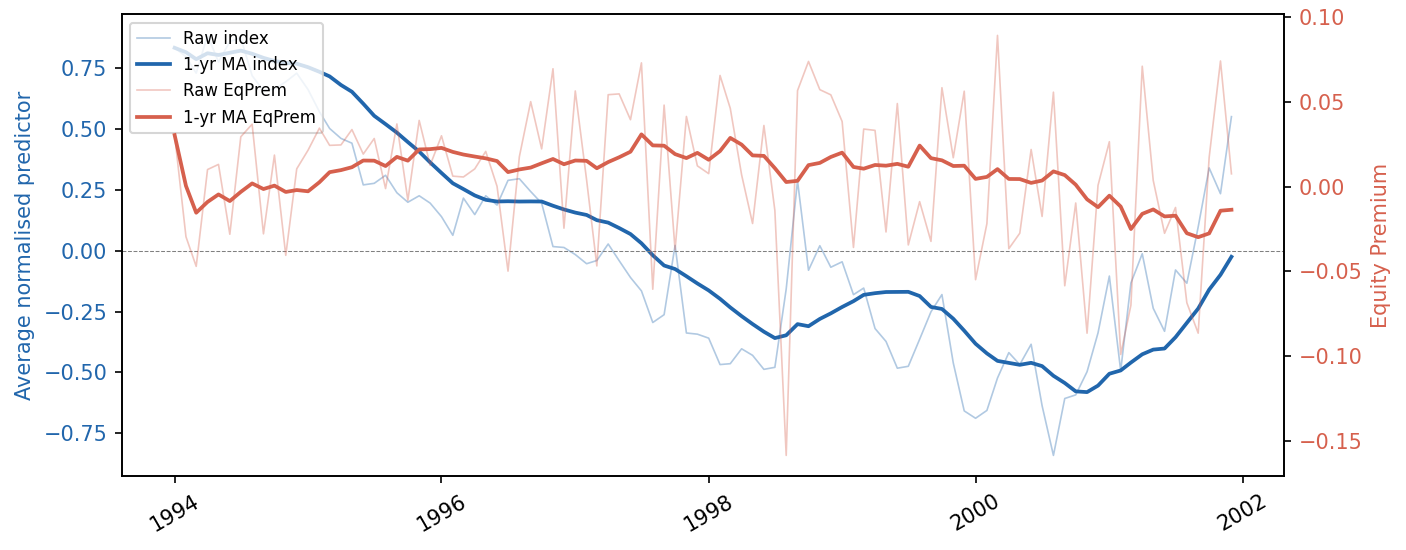
\includegraphics[width=\linewidth]{positive_index_monthly2.png}
    \caption{Positive predictor index}
\end{subfigure}
\hfill
\begin{subfigure}{0.85\textwidth}
    \centering
    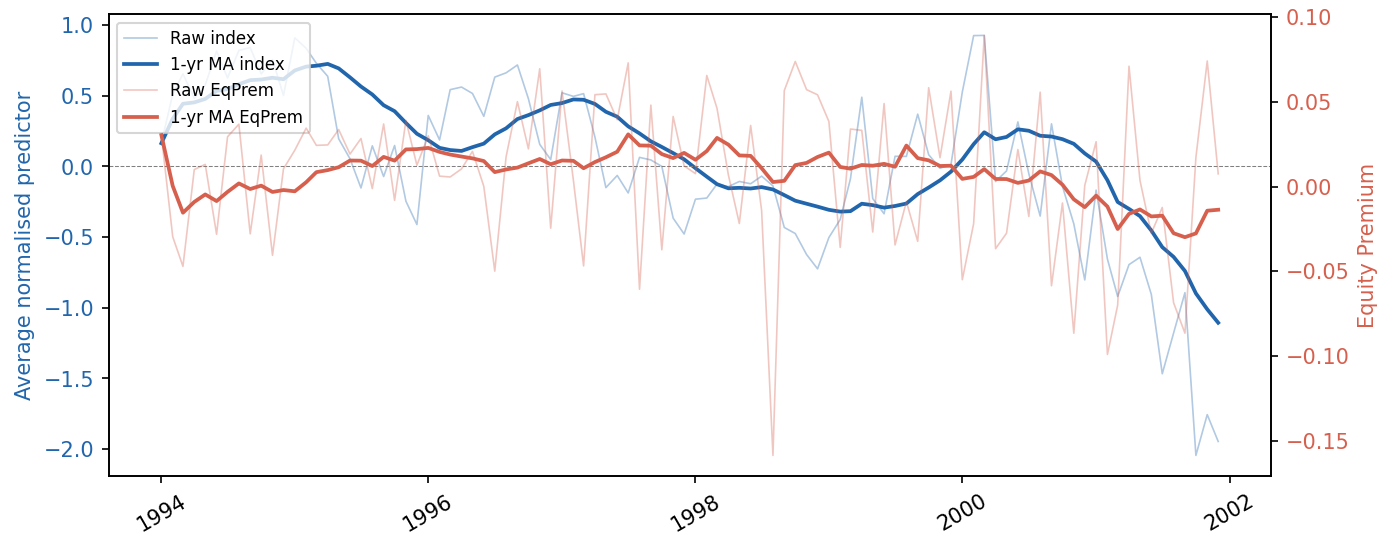
\includegraphics[width=\linewidth]{negative_index_monthly2.png}
    \caption{Negative predictor index}
\end{subfigure}

\caption{
Normalised predictors and the equity premium based on log returns sampled at monthly frequency from 1994-2001.
Each panel shows the average normalised predictor (left axis) and the log equity premium (right axis), including raw series and one-year moving averages.
}
\label{fig:quarterly_indices}
\end{figure}

\section{AIC and BIC for Out-of-Sample sPCA}\label{app:aic_bic}

\begin{table}[H]
\centering
\caption{AIC and BIC for sPCA specifications}
\label{tab:aic_bic_direct_spca_combined}
\small
\renewcommand{\arraystretch}{1.15}
\begin{tabular}{@{}llcccccc@{}}
\toprule
& & \multicolumn{3}{c}{Quarterly} & \multicolumn{3}{c}{Monthly} \\
\cmidrule(lr){3-5} \cmidrule(lr){6-8}
Restriction & Model 
& 1979--2022 & 1979--1993 & 1994--2022
& 1979--2022 & 1979--1993 & 1994--2022 \\
\midrule
\multicolumn{8}{@{}l}{\textit{Panel A: AIC -- Without \citet{campbellthompson2008} restrictions}} \\
& $K = 1$ 
& \textbf{-879.3} & \textbf{-303.6} & \textbf{-572.1}
& -3283.6 & -1112.4 & \textbf{-2167.2} \\
& $K = 2$ 
& -878.3 & -301.7 & -571.1
& -3280.0 & -1109.7 & -2164.3 \\
& $K = 3$ 
& -871.6 & -302.9 & -562.1
& \textbf{-3284.2} & \textbf{-1113.0} & -2163.2 \\
& $K = 4$ 
& -863.9 & -296.9 & -557.9
& -3268.9 & -1110.9 & -2148.0 \\
\multicolumn{8}{@{}l}{\textit{Panel B: AIC -- With \citet{campbellthompson2008} restrictions}} \\
& $K = 1$ 
& \textbf{-879.9} & -303.8 & \textbf{-572.6}
& -3283.8 & -1112.5 & \textbf{-2167.3} \\
& $K = 2$ 
& -878.9 & -303.0 & -570.5
& -3282.6 & -1109.6 & -2167.2 \\
& $K = 3$ 
& -876.3 & \textbf{-305.2} & -564.7
& \textbf{-3285.7} & \textbf{-1114.9} & -2162.8 \\
& $K = 4$ 
& -870.9 & -301.3 & -560.9
& -3277.8 & -1114.3 & -2153.5 \\
\midrule
\multicolumn{8}{@{}l}{\textit{Panel C: BIC -- Without \citet{campbellthompson2008} restrictions}} \\
& $K = 1$ 
& \textbf{-872.9} & \textbf{-299.4} & \textbf{-566.6}
& \textbf{-3275.1} & \textbf{-1106.1} & \textbf{-2159.5} \\
& $K = 2$ 
& -868.8 & -295.4 & -562.8
& -3267.2 & -1100.1 & -2152.8 \\
& $K = 3$ 
& -858.9 & -294.5 & -551.0
& -3267.1 & -1100.3 & -2147.8 \\
& $K = 4$ 
& -848.0 & -286.4 & -544.1
& -3247.6 & -1095.0 & -2128.7 \\
\multicolumn{8}{@{}l}{\textit{Panel D: BIC -- With \citet{campbellthompson2008} restrictions}} \\
& $K = 1$ 
& \textbf{-873.5} & \textbf{-299.6} & \textbf{-567.1}
& \textbf{-3275.2} & \textbf{-1106.1} & \textbf{-2159.6} \\
& $K = 2$ 
& -869.4 & -296.7 & -562.2
& -3269.8 & -1100.0 & -2155.6 \\
& $K = 3$ 
& -863.6 & -296.8 & -553.7
& -3268.6 & -1102.2 & -2147.3 \\
& $K = 4$ 
& -855.0 & -290.8 & -547.2
& -3256.5 & -1098.4 & -2134.3 \\
\bottomrule
\end{tabular}
\end{table}

\section{Factor Selection}
\begin{table}[H]
\centering
\caption{Expanding-Window AIC Factor Selection Frequency (\%)}
\label{tab:factor_selection}
\small
\renewcommand{\arraystretch}{1.15}
\begin{tabular}{@{}ll*{6}{S[table-format=3.1]}@{}}
\toprule
& & \multicolumn{3}{c}{Quarterly} & \multicolumn{3}{c}{Monthly} \\
\cmidrule(lr){3-5} \cmidrule(lr){6-8}
{Method} & {$K$}
& {1979--2022} & {1979--1993} & {1994--2022}
& {1979--2022} & {1979--1993} & {1994--2022} \\
\midrule
\multicolumn{8}{@{}l}{\textit{Panel A: Without CT restrictions}} \\
{sPCA direct}
  & {$K=1$} & 99.6 & 99.1 & 100.0 & 64.1 & 45.7 & 82.5 \\
  & {$K=3$} & 0.4  & 0.9  & {---} & 3.3  & 0.6  & 6.0 \\
  & {$K=4$} & {---}& {---}& {---} & 32.6 & 53.7 & 11.5 \\
\midrule
\multicolumn{8}{@{}l}{\textit{Panel B: With CT restrictions}} \\
{sPCA direct}
  & {$K=1$} & 100.0 & 100.0 & 100.0 & 35.8 & 61.2 & 10.3 \\
  & {$K=3$} & {---} & {---} & {---} & 33.6 & {---} & 67.2 \\
  & {$K=4$} & {---} & {---} & {---} & 30.6 & 38.8 & 22.4 \\
\bottomrule
\end{tabular}
\vspace{0.4em}
\begin{minipage}{0.85\textwidth}
\footnotesize
\textit{Notes:} Percentage of OOS periods in which each $K$ is selected by the AIC criterion using an expanding window. BIC selects $K=1$ in $\geq$99.6\% of periods across all specifications and is omitted. Only values of $K$ selected at least once are shown. CT refers to \citet{campbellthompson2008} restrictions.
\end{minipage}
\end{table}



\section{sPCA and DMFSE Weighting Scheme Performance}\label{app:spca_dmfse_performance}
\begin{table}[H]
\centering
\caption{$R^2_{OS}$ of sPCA for different factors (K = 1--4) and DMFSE Weighting Scheme}
\label{tab:spca_results_full_benchmarks}
\small
\begin{tabular}{lcccccc}
\hline
 & \multicolumn{3}{c}{Quarterly} & \multicolumn{3}{c}{Monthly} \\
\cmidrule(lr){2-4} \cmidrule(lr){5-7}
 & 1979--2022 & 1979--1993 & 1994--2022 
 & 1979--2022 & 1979--1993 & 1994--2022 \\
\cmidrule(lr){2-4} \cmidrule(lr){5-7}
Method 
& $R^2_{OS}$ & $R^2_{OS}$ & $R^2_{OS}$ 
& $R^2_{OS}$ & $R^2_{OS}$ & $R^2_{OS}$ \\
\hline
\multicolumn{7}{l}{\textit{Panel A: Without \citet{campbellthompson2008} restrictions}} \\[0.5ex]
1/N (RSZ) 
& \textbf{0.76}$^{*}$ & \textbf{2.62}$^{***}$ & -0.05 
& \textbf{0.16} & \textbf{0.72}$^{**}$ & -0.14 \\
\hline
sPCA direct ($K=1$) 
& -0.70 & -1.53 & -0.35 
& -0.36 & -0.58 & \textbf{-0.25} \\
sPCA direct ($K=2$) 
& \textbf{-0.08} & -1.35 & \textbf{0.47} 
& -0.68 & -0.99 & -0.51 \\
sPCA direct ($K=3$) 
& -2.83$^{*}$ & \textbf{3.88}$^{**}$ & -5.75 
& \textbf{0.50}$^{**}$ & \textbf{1.95}$^{**}$ & -0.27 \\
sPCA direct ($K=4$) 
& -6.22 & -2.71$^{*}$ & -7.74 
& -2.03$^{*}$ & 1.90$^{***}$ & -4.14 \\
\hline
sPCA-MVP ($K=1$) 
& -0.73 & 1.97 & -1.91 
& -0.14 & 0.31 & -0.38 \\
sPCA-MVP ($K=2$) 
& -0.24 & -0.05 & -0.32 
& \textbf{0.29} & 0.32 & \textbf{0.28} \\
sPCA-MVP ($K=3$) 
& -0.05 & 0.21 & -0.17 
& -0.03 & \textbf{0.76} & -0.45 \\
sPCA-MVP ($K=4$) 
& \textbf{1.38}$^{*}$ & \textbf{4.92}$^{**}$ & \textbf{-0.16} 
& 0.11 & 0.42 & -0.06 \\[1ex]
\multicolumn{7}{l}{\textit{Panel B: With \citet{campbellthompson2008} restrictions}} \\[0.5ex]
1/N (RSZ) 
& \textbf{0.90}$^{**}$ & \textbf{2.66}$^{***}$ & \textbf{0.13} 
& \textbf{0.23}$^{*}$ & \textbf{0.81}$^{**}$ & -0.08 \\
\hline
sPCA direct ($K=1$) 
& -0.35 & -1.22 & \textbf{0.02} 
& -0.33 & -0.55 & -0.22 \\
sPCA direct ($K=2$) 
& \textbf{0.23} & 0.84 & -0.04 
& -0.17 & -1.07 & \textbf{0.32} \\
sPCA direct ($K=3$) 
& -0.10 & \textbf{7.48}$^{***}$ & -3.40 
& \textbf{0.79}$^{**}$ & 2.99$^{***}$ & -0.39 \\
sPCA direct ($K=4$) 
& -2.06 & 4.57$^{**}$ & -4.95 
& -0.32$^{*}$ & \textbf{3.74}$^{***}$ & -2.50 \\
\hline
sPCA-MVP ($K=1$) 
& -0.08 & 2.72$^{*}$ & -1.30 
& 0.17 & 1.01$^{**}$ & -0.28 \\
sPCA-MVP ($K=2$) 
& -0.55 & -0.07 & -0.76 
& \textbf{0.33}$^{*}$ & \textbf{1.02}$^{*}$ & \textbf{-0.05} \\
sPCA-MVP ($K=3$) 
& 0.11 & -0.05 & 0.18 
& 0.19 & 1.01$^{**}$ & -0.25 \\
sPCA-MVP ($K=4$) 
& \textbf{1.77}$^{**}$ & \textbf{4.74}$^{**}$ & \textbf{0.47} 
& 0.24 & 1.01$^{**}$ & -0.17 \\
\hline
\multicolumn{7}{p{0.85\textwidth}}{\footnotesize \textit{Notes:} The table reports out-of-sample $R^2_{OS}$ values (in \%) without or with restrictions from \citet{campbellthompson2008}. The subsamples correspond to
1979--1993 (pre-1994) and 1994--2022 (post-1994). Statistical significance is
assessed using Clark and West (2007) test. $^{*}p < 0.10$, $^{**}p < 0.05$, $^{***}p < 0.01$. $1/N$ RSZ is the \citet{rsz2010} equal weighted combination.} 
\end{tabular}
\end{table}

\begin{table}[H]
\centering
\caption{Annualised CER Gains, Confidence Intervals and Break-Even Trading Costs for Out-of-Sample sPCA and DMSFE Forecasts: Expanding Window}
\label{tab:cer_expanding}
\footnotesize
\setlength{\tabcolsep}{2pt}
\begin{tabular}{@{}l
    >{\centering\arraybackslash}p{1.0cm}
    >{\centering\arraybackslash}p{2.0cm}
    >{\centering\arraybackslash}p{1.0cm}
    @{\hspace{4pt}\vrule\hspace{4pt}}
    >{\centering\arraybackslash}p{1.0cm}
    >{\centering\arraybackslash}p{2.0cm}
    >{\centering\arraybackslash}p{1.0cm}
    @{\hspace{4pt}\vrule\hspace{4pt}}
    >{\centering\arraybackslash}p{1.0cm}
    >{\centering\arraybackslash}p{2.0cm}
    >{\centering\arraybackslash}p{1.0cm}@{}}
\toprule
& \multicolumn{3}{c}{1979--2022} & \multicolumn{3}{c}{1979--1993} & \multicolumn{3}{c}{1994--2022} \\
\cmidrule(r){2-4}\cmidrule(lr){5-7}\cmidrule(l){8-10}
Method & CER & {\scriptsize [90\% CI]} & TC$^{\dagger}$
        & CER & {\scriptsize [90\% CI]} & TC$^{\dagger}$
        & CER & {\scriptsize [90\% CI]} & TC$^{\dagger}$ \\
\midrule

\multicolumn{10}{@{}l}{\textit{Panel A: Quarterly -- Without \citet{campbellthompson2008} restrictions}} \\
1/N
  & 49.3 & {\scriptsize [$-$36.4, 133.1]} & 244.3
  & 151.8 & {\scriptsize [57.8, 258.9]} & 554.0
  & $-$3.7 & {\scriptsize [$-$116.4, 105.9]} & $-$22.5 \\
sPCA ($K=1$)
  & $-$8.0 & {\scriptsize [$-$111.8, 107.7]} & $-$56.7
  & $-$22.5 & {\scriptsize [$-$136.1, 81.1]} & $-$97.5
  & $-$0.3 & {\scriptsize [$-$156.2, 181.6]} & $-$3.3 \\
sPCA ($K=2$)
  & $-$57.9 & {\scriptsize [$-$487.7, 305.9]} & $-$150.1
  & $-$125.9 & {\scriptsize [$-$587.4, 344.3]} & $-$627.9
  & $-$20.4 & {\scriptsize [$-$577.4, 574.8]} & $-$42.4 \\
sPCA ($K=3$)
  & 127.9 & {\scriptsize [$-$251.3, 470.9]} & 210.2
  & 490.5 & {\scriptsize [163.9, 818.1]} & 517.6
  & $-$55.1 & {\scriptsize [$-$550.5, 417.4]} & $-$132.4 \\
sPCA ($K=4$)
  & $-$39.5 & {\scriptsize [$-$408.2, 291.7]} & $-$50.9
  & 148.2 & {\scriptsize [$-$184.2, 498.6]} & 135.5
  & $-$135.2 & {\scriptsize [$-$655.0, 376.0]} & $-$220.7 \\
sPCA (best AIC)
  & $-$8.0 & {\scriptsize [$-$111.8, 107.7]} & $-$56.7
  & $-$22.5 & {\scriptsize [$-$136.1, 81.1]} & $-$97.5
  & $-$0.3 & {\scriptsize [$-$156.2, 181.6]} & $-$3.3 \\[0.3ex]
DMSFE ($\delta=0.95$)
  & 42.8 & {\scriptsize [$-$36.8, 122.3]} & 173.6
  & 129.9 & {\scriptsize [41.0, 233.9]} & 328.0
  & $-$2.5 & {\scriptsize [$-$109.3, 100.5]} & $-$14.4 \\
DMSFE ($\delta=0.99$)
  & 43.7 & {\scriptsize [$-$38.9, 124.4]} & 177.7
  & 133.8 & {\scriptsize [44.4, 237.7]} & 339.1
  & $-$3.0 & {\scriptsize [$-$113.4, 105.3]} & $-$17.4 \\
DMSFE ($\delta=1.00$)
  & 44.7 & {\scriptsize [$-$38.2, 125.9]} & 181.5
  & 134.7 & {\scriptsize [44.8, 238.6]} & 341.7
  & $-$1.9 & {\scriptsize [$-$112.9, 107.8]} & $-$11.2 \\[1ex]

\multicolumn{10}{@{}l}{\textit{Panel B: Quarterly -- With \citet{campbellthompson2008} restrictions}} \\
1/N
  & 56.9 & {\scriptsize [$-$30.0, 137.7]} & 296.0
  & 153.9 & {\scriptsize [59.2, 262.9]} & 571.2
  & 6.6 & {\scriptsize [$-$98.6, 115.2]} & 42.8 \\
sPCA ($K=1$)
  & 12.7 & {\scriptsize [$-$93.0, 134.2]} & 93.0
  & $-$7.3 & {\scriptsize [$-$107.3, 84.0]} & $-$34.4
  & 23.2 & {\scriptsize [$-$135.2, 203.0]} & 236.8 \\
sPCA ($K=2$)
  & $-$23.2 & {\scriptsize [$-$451.6, 321.6]} & $-$57.8
  & $-$106.5 & {\scriptsize [$-$588.9, 377.9]} & $-$426.0
  & 22.1 & {\scriptsize [$-$519.6, 576.8]} & 45.8 \\
sPCA ($K=3$)
  & 102.5 & {\scriptsize [$-$271.4, 449.8]} & 157.1
  & 477.3 & {\scriptsize [152.2, 798.6]} & 477.2
  & $-$86.6 & {\scriptsize [$-$580.5, 394.1]} & $-$189.7 \\
sPCA ($K=4$)
  & $-$47.2 & {\scriptsize [$-$417.3, 294.3]} & $-$58.2
  & 148.0 & {\scriptsize [$-$183.3, 496.2]} & 133.7
  & $-$146.5 & {\scriptsize [$-$676.6, 369.8]} & $-$222.4 \\
sPCA (best AIC)
  & 12.7 & {\scriptsize [$-$93.0, 134.2]} & 93.0
  & $-$7.3 & {\scriptsize [$-$107.3, 84.0]} & $-$34.4
  & 23.2 & {\scriptsize [$-$135.2, 203.0]} & 236.8 \\[0.3ex]
DMSFE ($\delta=0.95$)
  & 50.0 & {\scriptsize [$-$28.5, 127.0]} & 211.0
  & 131.7 & {\scriptsize [41.6, 236.8]} & 335.9
  & 7.5 & {\scriptsize [$-$92.5, 110.9]} & 47.2 \\
DMSFE ($\delta=0.99$)
  & 50.9 & {\scriptsize [$-$30.6, 130.7]} & 215.1
  & 135.6 & {\scriptsize [45.1, 242.8]} & 347.2
  & 6.9 & {\scriptsize [$-$97.0, 114.9]} & 43.6 \\
DMSFE ($\delta=1.00$)
  & 51.9 & {\scriptsize [$-$30.2, 131.4]} & 218.9
  & 136.5 & {\scriptsize [45.8, 244.6]} & 349.8
  & 7.9 & {\scriptsize [$-$96.5, 117.2]} & 49.6 \\[1ex]

\midrule

\multicolumn{10}{@{}l}{\textit{Panel C: Monthly -- Without \citet{campbellthompson2008} restrictions}} \\
1/N
  & 33.8 & {\scriptsize [$-$38.8, 111.1]} & 44.4
  & 145.1 & {\scriptsize [30.3, 275.4]} & 158.1
  & $-$23.7 & {\scriptsize [$-$120.6, 62.3]} & $-$34.7 \\
sPCA ($K=1$)
  & $-$57.4 & {\scriptsize [$-$178.3, 78.3]} & $-$264.3
  & $-$89.9 & {\scriptsize [$-$210.2, 33.9]} & $-$321.3
  & $-$40.5 & {\scriptsize [$-$223.6, 164.0]} & $-$219.0 \\
sPCA ($K=2$)
  & $-$133.7 & {\scriptsize [$-$454.1, 211.6]} & $-$270.6
  & $-$319.6 & {\scriptsize [$-$835.2, 238.2]} & $-$15327.8
  & $-$36.1 & {\scriptsize [$-$446.0, 390.9]} & $-$48.9 \\
sPCA ($K=3$)
  & 252.2 & {\scriptsize [$-$44.1, 536.2]} & 82.0
  & 662.6 & {\scriptsize [233.7, 1080.2]} & 229.7
  & 42.2 & {\scriptsize [$-$327.7, 384.1]} & 13.3 \\
sPCA ($K=4$)
  & 36.8 & {\scriptsize [$-$282.1, 340.3]} & 20.1
  & 611.3 & {\scriptsize [230.8, 980.3]} & 272.5
  & $-$256.2 & {\scriptsize [$-$703.3, 128.9]} & $-$159.4 \\
sPCA (best AIC)
  & 106.5 & {\scriptsize [$-$125.0, 346.5]} & 95.9
  & 521.8 & {\scriptsize [164.9, 860.9]} & 256.5
  & $-$105.1 & {\scriptsize [$-$389.9, 173.5]} & $-$168.5 \\[0.3ex]
DMSFE ($\delta=0.95$)
  & 29.5 & {\scriptsize [$-$38.9, 106.7]} & 37.4
  & 124.8 & {\scriptsize [10.8, 255.8]} & 129.0
  & $-$19.7 & {\scriptsize [$-$113.3, 64.9]} & $-$28.2 \\
DMSFE ($\delta=0.99$)
  & 28.3 & {\scriptsize [$-$42.3, 105.5]} & 36.4
  & 130.0 & {\scriptsize [14.3, 261.8]} & 136.4
  & $-$24.3 & {\scriptsize [$-$119.5, 60.8]} & $-$35.3 \\
DMSFE ($\delta=1.00$)
  & 28.7 & {\scriptsize [$-$43.2, 105.2]} & 37.0
  & 131.3 & {\scriptsize [15.1, 263.0]} & 138.0
  & $-$24.4 & {\scriptsize [$-$120.5, 61.7]} & $-$35.6 \\[1ex]

\multicolumn{10}{@{}l}{\textit{Panel D: Monthly -- With \citet{campbellthompson2008} restrictions}} \\
1/N
  & 38.4 & {\scriptsize [$-$36.7, 114.4]} & 55.3
  & 164.4 & {\scriptsize [50.4, 296.0]} & 192.0
  & $-$26.7 & {\scriptsize [$-$119.6, 61.4]} & $-$43.6 \\
sPCA ($K=1$)
  & $-$50.9 & {\scriptsize [$-$164.2, 76.6]} & $-$227.2
  & $-$77.9 & {\scriptsize [$-$193.6, 42.4]} & $-$298.5
  & $-$36.9 & {\scriptsize [$-$208.6, 151.4]} & $-$179.9 \\
sPCA ($K=2$)
  & $-$66.7 & {\scriptsize [$-$374.2, 256.6]} & $-$149.3
  & $-$318.7 & {\scriptsize [$-$834.2, 241.9]} & $-$9607.8
  & 65.7 & {\scriptsize [$-$319.3, 418.9]} & 99.5 \\
sPCA ($K=3$)
  & 319.0 & {\scriptsize [$-$8.4, 626.2]} & 89.1
  & 607.9 & {\scriptsize [199.7, 1021.2]} & 221.0
  & 171.1 & {\scriptsize [$-$242.1, 579.4]} & 42.8 \\
sPCA ($K=4$)
  & 74.9 & {\scriptsize [$-$239.7, 390.5]} & 30.6
  & 585.9 & {\scriptsize [204.4, 941.1]} & 239.8
  & $-$186.4 & {\scriptsize [$-$606.5, 231.1]} & $-$76.2 \\
sPCA (best AIC)
  & 239.6 & {\scriptsize [$-$80.2, 537.4]} & 87.8
  & 469.4 & {\scriptsize [120.2, 806.1]} & 231.7
  & 122.7 & {\scriptsize [$-$362.0, 544.8]} & 39.8 \\[0.3ex]
DMSFE ($\delta=0.95$)
  & 34.4 & {\scriptsize [$-$36.8, 108.6]} & 47.6
  & 143.9 & {\scriptsize [29.1, 276.4]} & 158.5
  & $-$22.2 & {\scriptsize [$-$111.2, 61.9]} & $-$35.4 \\
DMSFE ($\delta=0.99$)
  & 33.0 & {\scriptsize [$-$40.9, 107.1]} & 46.5
  & 149.1 & {\scriptsize [34.0, 282.6]} & 167.0
  & $-$27.1 & {\scriptsize [$-$118.3, 58.8]} & $-$44.0 \\
DMSFE ($\delta=1.00$)
  & 33.3 & {\scriptsize [$-$41.9, 107.9]} & 46.9
  & 150.3 & {\scriptsize [34.9, 282.9]} & 168.9
  & $-$27.3 & {\scriptsize [$-$119.7, 60.1]} & $-$44.4 \\
\bottomrule
\end{tabular}
\vspace{0.4em}
\begin{minipage}{\textwidth}
\footnotesize
\textit{Notes:} CER gains are annualised and expressed in basis points, computed as in equation (\ref{eq:utility}). 90\% CI reports the bootstrap confidence interval. sPCA (best AIC) selects $K$ at each OOS step via expanding-window AIC. DMSFE combines forecasts using discounted mean squared forecast error weights. \citet{campbellthompson2008} refers to Campbell \& Thompson (2008) sign restrictions on the equity premium forecast and portfolio weight. $^{\dagger}$TC denotes the breakeven transaction cost in annualised basis points.
\end{minipage}
\end{table}

\section{Individual correlation plots}
\subsection{Monthly unrestricted}
\begin{figure}[H]
    \centering
    
\includegraphics[width=1 \linewidth]{Paper final Joost Copy/individual_predictor_corr_monthly_unrestricted_W60.png}
    \caption{Enter Caption}
    \label{fig:placeholder}
\end{figure}

\begin{figure}[H]
    \centering
    
\includegraphics[width= 1\linewidth]{Paper final Joost Copy/individual_predictor_corr_monthly_restricted_W120.png}
    \caption{Enter Caption}
    \label{fig:placeholder}
\end{figure}

\begin{figure}[H]
    \centering
    
\includegraphics[width= 1\linewidth]{Paper final Joost Copy/individual_predictor_corr_monthly_unrestricted_W180.png}
    \caption{Enter Caption}
    \label{fig:placeholder}
\end{figure}

\newpage
\subsection{Monthly restricted}
\begin{figure}[H]
    \centering
    
\includegraphics[width=1\linewidth]{Paper final Joost Copy/individual_predictor_corr_monthly_restricted_W60.png}
    \caption{Enter Caption}
    \label{fig:placeholder}
\end{figure}

\begin{figure}[H]
    \centering
    
\includegraphics[width=1\linewidth]{Paper final Joost Copy/individual_predictor_corr_monthly_restricted_W120.png}
    \caption{Enter Caption}
    \label{fig:placeholder}
\end{figure}

\begin{figure}[H]
    \centering
    
\includegraphics[width=1\linewidth]{Paper final Joost Copy/individual_predictor_corr_monthly_restricted_W180.png}
    \caption{Enter Caption}
    \label{fig:placeholder}
\end{figure}

\newpage
\subsection{Quarterly Unrestricted}

\begin{figure}[H]
    \centering
    
\includegraphics[width=1 \linewidth]{Paper final Joost Copy/individual_predictor_corr_quarterly_unrestricted_W20.png}
    \caption{Enter Caption}
    \label{fig:placeholder}
\end{figure}

\begin{figure}[H]
    \centering
    
\includegraphics[width= 1\linewidth]{Paper final Joost Copy/individual_predictor_corr_quarterly_unrestricted_W40.png}
    \caption{Enter Caption}
    \label{fig:placeholder}
\end{figure}

\begin{figure}[H]
    \centering
    
\includegraphics[width= 1\linewidth]{Paper final Joost Copy/individual_predictor_corr_quarterly_unrestricted_W60.png}
    \caption{Enter Caption}
    \label{fig:placeholder}
\end{figure}

\newpage
\subsection{Quarterly Restricted}

\begin{figure}[H]
    \centering
    
\includegraphics[width=1 \linewidth]{Paper final Joost Copy/individual_predictor_corr_quarterly_restricted_W20.png}
    \caption{Enter Caption}
    \label{fig:placeholder}
\end{figure}

\begin{figure}[H]
    \centering
    
\includegraphics[width= 1\linewidth]{Paper final Joost Copy/individual_predictor_corr_quarterly_restricted_W40.png}
    \caption{Enter Caption}
    \label{fig:placeholder}
\end{figure}

\begin{figure}[H]
    \centering
    
\includegraphics[width= 1\linewidth]{Paper final Joost Copy/individual_predictor_corr_quarterly_restricted_W60.png}
    \caption{Enter Caption}
    \label{fig:placeholder}
\end{figure}


\section{$S^{fr}_t$ Plots for Different Values of $\lambda$ for Distributed OLS}

\begin{figure}[H]
    \centering
    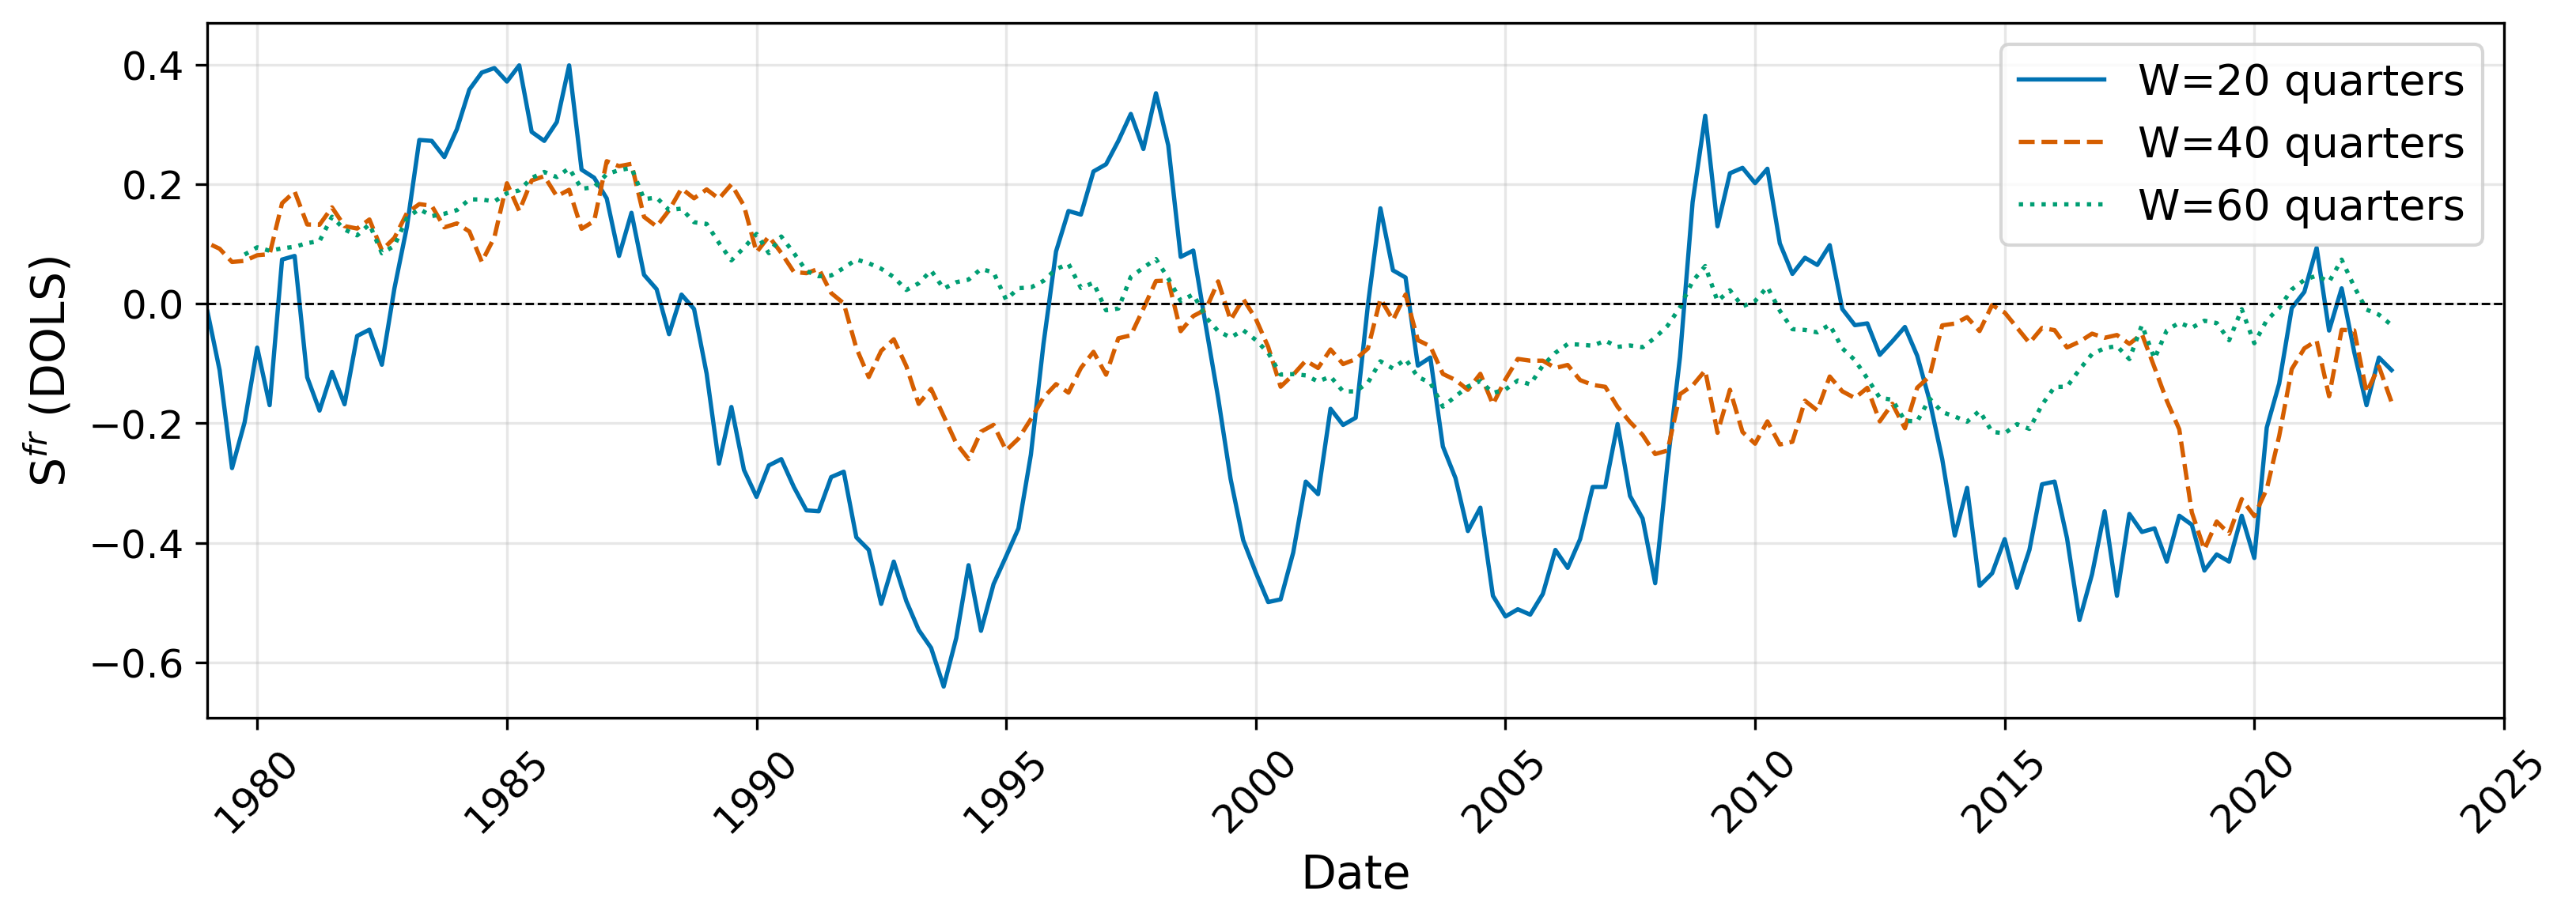
\includegraphics[width=0.85\linewidth]{plot_DOLS_S_fr_delta96594_quarterly_unrestricted.png}
    \caption{Quarterly $S^{fr}_t$ plot for $\delta = 0.96594$}
    \label{fig:quarterly1}
\end{figure}

\begin{figure}[H]
    \centering
    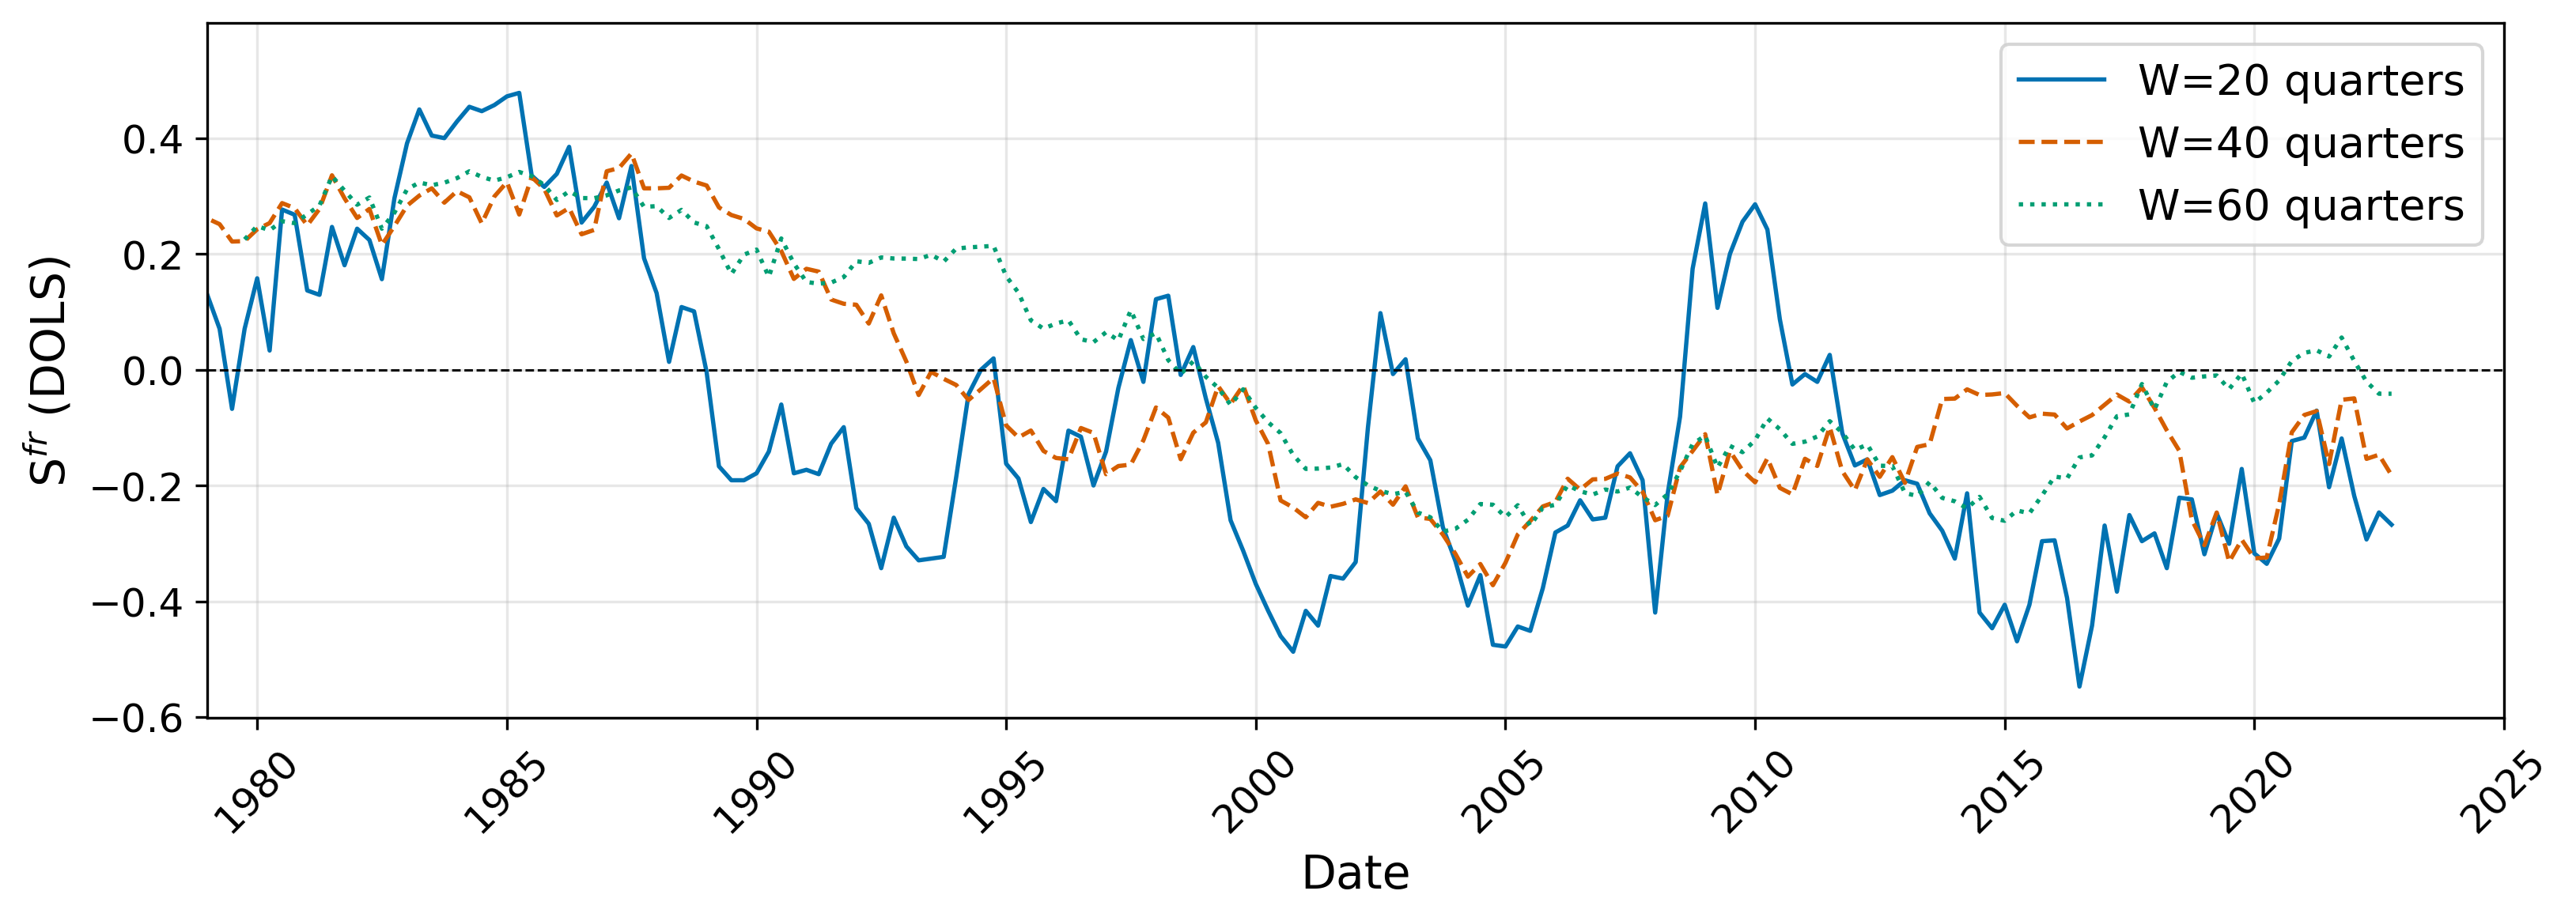
\includegraphics[width=0.85\linewidth]{plot_DOLS_S_fr_delta98851_quarterly_unrestricted.png}
    \caption{Quarterly $S^{fr}_t$ plot for $\delta = 0.99951$}
    \label{fig:quaerterly3}
\end{figure}

\begin{figure}[H]
    \centering
    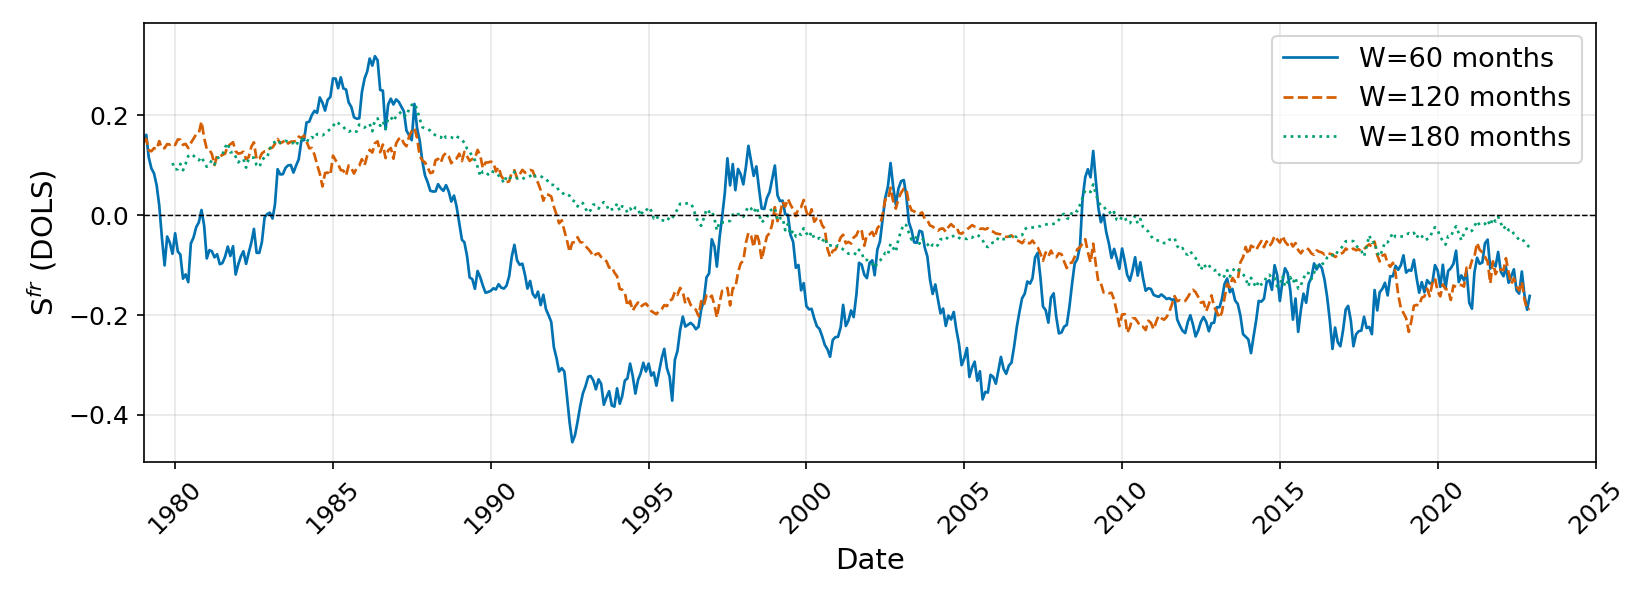
\includegraphics[width=0.85\linewidth]{plot_DOLS_S_fr_delta98851_monthly_unrestricted.png}
    \caption{Monthly $S^{fr}_t$ plot for $\delta = 0.98851$}
    \label{fig:monthly1}
\end{figure}

\begin{figure}[H]
    \centering
    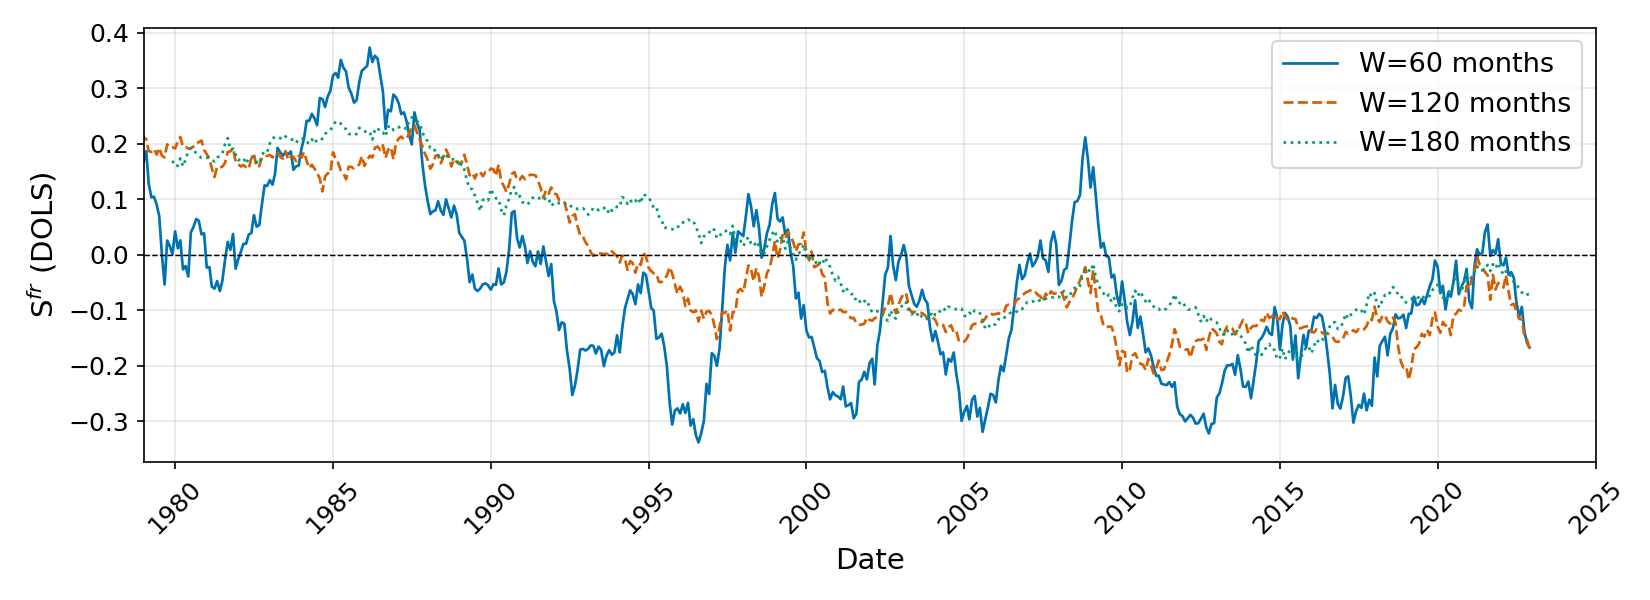
\includegraphics[width=0.85\linewidth]{plot_DOLS_S_fr_delta99616_monthly_unrestricted.png}
    \caption{Monthly $S^{fr}_t$ plot for $\delta = 0.99616$}
    \label{fig:monthly3}
\end{figure}

\section{Discounting Parameter $\lambda$ Values}\label{app:disc_lambda}

\begin{table}[H]
\centering
\caption{Discounting Parameters Across Window Lengths}
\label{tab:discounted_lambda}
\small
\begin{tabular}{lcc}
\hline
 & Quarterly & Monthly \\
\cmidrule(lr){2-2} \cmidrule(lr){3-3}
Window & $\lambda$ & $\lambda$ \\
\hline
5-year  & 0.96594 & 0.98851 \\
10-year & 0.98282 & 0.99424 \\
15-year & 0.98851 & 0.99616\\
\hline
\end{tabular}
\end{table}

\section{CER Gain for Rolling Window and D-OLS}\label{app:cer_rol_dols}
\begin{table}[H]
\centering
\caption{Annualised CER Gains, Confidence Intervals and Break-Even Trading Costs for Out-of-Sample Rolling Window and D-OLS}
\label{tab:cer_gains_combined2}
\footnotesize
\setlength{\tabcolsep}{2pt}
\begin{tabular}{@{}l
    >{\centering\arraybackslash}p{1.0cm}
    >{\centering\arraybackslash}p{2.0cm}
    >{\centering\arraybackslash}p{1.0cm}
    @{\hspace{4pt}\vrule\hspace{4pt}}
    >{\centering\arraybackslash}p{1.0cm}
    >{\centering\arraybackslash}p{2.0cm}
    >{\centering\arraybackslash}p{1.0cm}
    @{\hspace{4pt}\vrule\hspace{4pt}}
    >{\centering\arraybackslash}p{1.0cm}
    >{\centering\arraybackslash}p{2.0cm}
    >{\centering\arraybackslash}p{1.0cm}@{}}
\toprule
& \multicolumn{3}{c}{1979--2022} & \multicolumn{3}{c}{1979--1993} & \multicolumn{3}{c}{1994--2022} \\
\cmidrule(r){2-4}\cmidrule(lr){5-7}\cmidrule(l){8-10}
Method & CER & {\scriptsize [90\% CI]} & TC$^{\dagger}$
        & CER & {\scriptsize [90\% CI]} & TC$^{\dagger}$
        & CER & {\scriptsize [90\% CI]} & TC$^{\dagger}$ \\
\midrule

\multicolumn{10}{@{}l}{\textit{Panel A: Quarterly -- Without \citet{campbellthompson2008} restrictions}} \\
Rolling (1/N) (5y)
  & $-$80.7 & {\scriptsize [$-$277.7, 124.1]} & $-$127.9
  & $-$203.5 & {\scriptsize [$-$482.4, 98.7]} & $-$225.0
  & $-$16.7 & {\scriptsize [$-$267.5, 271.7]} & $-$33.8 \\
Rolling (1/N) (10y)
  & $-$90.7 & {\scriptsize [$-$273.7, 101.3]} & $-$204.8
  & $-$181.2 & {\scriptsize [$-$457.8, 114.7]} & $-$307.6
  & $-$42.5 & {\scriptsize [$-$281.2, 249.1]} & $-$115.0 \\
Rolling (1/N) (15y)
  & $-$14.3 & {\scriptsize [$-$213.9, 197.8]} & $-$37.1
  & $-$52.9 & {\scriptsize [$-$410.9, 341.0]} & $-$97.4
  & 8.7 & {\scriptsize [$-$225.7, 284.9]} & 28.1 \\[0.3ex]
dOLS ($\delta=0.966$)
  & $-$31.3 & {\scriptsize [$-$155.0, 105.6]} & $-$99.5
  & $-$131.0 & {\scriptsize [$-$328.3, 47.2]} & $-$313.5
  & 21.1 & {\scriptsize [$-$136.6, 214.9]} & 80.3 \\
dOLS ($\delta=0.983$)
  & $-$43.2 & {\scriptsize [$-$128.6, 51.5]} & $-$179.0
  & 21.1 & {\scriptsize [$-$90.4, 138.2]} & 67.4
  & $-$76.3 & {\scriptsize [$-$185.8, 59.3]} & $-$371.4 \\
dOLS ($\delta=0.989$)
  & $-$34.7 & {\scriptsize [$-$109.3, 42.4]} & $-$157.6
  & 67.6 & {\scriptsize [$-$36.4, 174.0]} & 233.1
  & $-$87.4 & {\scriptsize [$-$173.1, 14.9]} & $-$472.4 \\[1ex]

\multicolumn{10}{@{}l}{\textit{Panel B: Quarterly -- With \citet{campbellthompson2008} restrictions}} \\
Rolling (1/N) (5y)
  & $-$291.7 & {\scriptsize [$-$533.7, $-$63.5]} & $-$383.0
  & $-$245.4 & {\scriptsize [$-$624.2, 185.8]} & $-$337.8
  & $-$315.7 & {\scriptsize [$-$653.6, $-$30.3]} & $-$402.1 \\
Rolling (1/N) (10y)
  & $-$168.4 & {\scriptsize [$-$350.1, 8.4]} & $-$361.4
  & $-$203.4 & {\scriptsize [$-$508.2, 136.2]} & $-$328.1
  & $-$149.2 & {\scriptsize [$-$381.0, 59.2]} & $-$382.6 \\
Rolling (1/N) (15y)
  & $-$115.1 & {\scriptsize [$-$269.0, 40.3]} & $-$297.3
  & $-$53.6 & {\scriptsize [$-$448.9, 373.3]} & $-$95.2
  & $-$144.4 & {\scriptsize [$-$275.5, $-$20.3]} & $-$482.1 \\[0.3ex]
dOLS ($\delta=0.966$)
  & $-$34.1 & {\scriptsize [$-$137.0, 75.0]} & $-$114.2
  & $-$142.4 & {\scriptsize [$-$372.9, 63.0]} & $-$358.5
  & 22.9 & {\scriptsize [$-$98.0, 153.8]} & 92.3 \\
dOLS ($\delta=0.983$)
  & $-$34.1 & {\scriptsize [$-$106.6, 39.1]} & $-$147.0
  & 22.1 & {\scriptsize [$-$89.6, 140.2]} & 71.3
  & $-$63.0 & {\scriptsize [$-$155.8, 39.8]} & $-$326.5 \\
dOLS ($\delta=0.989$)
  & $-$25.8 & {\scriptsize [$-$96.2, 43.4]} & $-$121.8
  & 68.9 & {\scriptsize [$-$35.7, 176.8]} & 241.0
  & $-$74.7 & {\scriptsize [$-$154.5, 11.4]} & $-$427.2 \\[1ex]

\midrule

\multicolumn{10}{@{}l}{\textit{Panel C: Monthly -- Without \citet{campbellthompson2008} restrictions}} \\
Rolling (1/N) (5y)
  & $-$125.9 & {\scriptsize [$-$367.5, 142.5]} & $-$84.9
  & $-$244.0 & {\scriptsize [$-$571.9, 106.7]} & $-$121.0
  & $-$64.9 & {\scriptsize [$-$382.1, 291.4]} & $-$53.6 \\
Rolling (1/N) (10y)
  & $-$79.6 & {\scriptsize [$-$315.8, 180.5]} & $-$76.0
  & $-$147.9 & {\scriptsize [$-$466.4, 195.8]} & $-$107.9
  & $-$43.8 & {\scriptsize [$-$375.6, 331.4]} & $-$49.8 \\
Rolling (1/N) (15y)
  & $-$10.5 & {\scriptsize [$-$214.8, 219.9]} & $-$10.8
  & $-$72.3 & {\scriptsize [$-$398.3, 272.9]} & $-$58.7
  & 22.5 & {\scriptsize [$-$263.8, 355.1]} & 26.8 \\[0.3ex]
dOLS ($\delta=0.989$)
  & $-$27.8 & {\scriptsize [$-$182.8, 153.2]} & $-$32.3
  & $-$120.4 & {\scriptsize [$-$345.8, 93.7]} & $-$110.0
  & 20.3 & {\scriptsize [$-$198.7, 252.8]} & 27.4 \\
dOLS ($\delta=0.994$)
  & $-$28.1 & {\scriptsize [$-$124.0, 84.9]} & $-$38.6
  & 23.9 & {\scriptsize [$-$82.5, 147.6]} & 29.0
  & $-$54.8 & {\scriptsize [$-$202.4, 106.5]} & $-$80.9 \\
dOLS ($\delta=0.996$)
  & $-$22.7 & {\scriptsize [$-$105.1, 64.8]} & $-$31.0
  & 74.7 & {\scriptsize [$-$28.4, 193.0]} & 94.1
  & $-$72.9 & {\scriptsize [$-$185.9, 49.9]} & $-$104.3 \\[1ex]

\multicolumn{10}{@{}l}{\textit{Panel D: Monthly -- With \citet{campbellthompson2008} restrictions}} \\
Rolling (1/N) (5y)
  & $-$166.8 & {\scriptsize [$-$375.7, 55.7]} & $-$138.1
  & $-$123.1 & {\scriptsize [$-$437.5, 188.1]} & $-$74.9
  & $-$189.6 & {\scriptsize [$-$485.3, 79.8]} & $-$193.0 \\
Rolling (1/N) (10y)
  & $-$82.6 & {\scriptsize [$-$265.2, 98.2]} & $-$87.6
  & $-$124.4 & {\scriptsize [$-$448.1, 224.3]} & $-$96.3
  & $-$60.6 & {\scriptsize [$-$276.7, 141.8]} & $-$79.4 \\
Rolling (1/N) (15y)
  & $-$110.9 & {\scriptsize [$-$243.4, 34.6]} & $-$132.5
  & $-$54.1 & {\scriptsize [$-$388.8, 304.2]} & $-$45.9
  & $-$139.5 & {\scriptsize [$-$286.3, $-$11.3]} & $-$210.6 \\[0.3ex]
dOLS ($\delta=0.989$)
  & $-$37.1 & {\scriptsize [$-$166.9, 82.9]} & $-$50.2
  & $-$120.6 & {\scriptsize [$-$364.8, 114.0]} & $-$115.7
  & 6.3 & {\scriptsize [$-$128.8, 146.3]} & 10.7 \\
dOLS ($\delta=0.994$)
  & $-$32.6 & {\scriptsize [$-$103.8, 40.9]} & $-$51.1
  & 34.9 & {\scriptsize [$-$68.9, 156.4]} & 43.5
  & $-$67.4 & {\scriptsize [$-$166.3, 32.8]} & $-$122.0 \\
dOLS ($\delta=0.996$)
  & $-$23.5 & {\scriptsize [$-$83.0, 41.6]} & $-$36.7
  & 87.8 & {\scriptsize [$-$13.2, 203.7]} & 115.4
  & $-$81.0 & {\scriptsize [$-$160.4, $-$7.1]} & $-$140.0 \\
\bottomrule
\end{tabular}
\vspace{0.4em}
\begin{minipage}{\textwidth}
\footnotesize
\textit{Notes:} CER gains are annualised and expressed in basis points, computed as in equation (\ref{eq:utility}). 90\% CI reports the bootstrap confidence interval. Rolling (1/N) uses equal-weighted portfolios with 5-, 10-, and 15-year estimation windows. dOLS denotes discounted OLS; quarterly data use $\delta\in\{0.966,0.983,0.989\}$ and monthly data use $\delta\in\{0.989,0.994,0.996\}$. \citet{campbellthompson2008} refers to Campbell \& Thompson (2008) sign restrictions on the equity premium forecast. $^{\dagger}$TC denotes the breakeven transaction cost in annualised basis points.
\end{minipage}
\end{table}

\end{document}
